 \documentclass[a4paper]{article}
\usepackage[utf8]{inputenc}
\usepackage{geometry}
\usepackage{graphicx}

\usepackage[T1]{fontenc}
\usepackage{lmodern}
\usepackage[ngerman]{babel}

\usepackage{float}

\usepackage{subfig}
\usepackage{wrapfig}


\usepackage[colorlinks,
pdfpagelabels,
pdfstartview = FitH,
bookmarksopen = true,
bookmarksnumbered = true,
linkcolor = black,
plainpages = false,
hypertexnames = false,
citecolor = black] {hyperref}

\usepackage{color}
\usepackage{xcolor}
\usepackage{listings}

\usepackage{caption}
\DeclareCaptionFont{white}{\color{white}}
\DeclareCaptionFormat{listing}{\colorbox{gray}{\parbox{\textwidth}{#1#2#3}}}
\captionsetup[lstlisting]{format=listing,labelfont=white,textfont=white}



\usepackage[nottoc]{tocbibind}

\title{Projektdokumenation\\Web-basierte Anwendungen\\Verteilte Systeme}
\author{Dennis Meyer\\Dominik Schilling}
\date{\today}

\begin{document}

\maketitle

\newpage

\tableofcontents

\newpage


\section{Einleitung}
Im Rahmen der zweiten Projektphase des Moduls Webbasierte Anwendungen 2: Verteilte Systeme, geht es um die Entwicklung einer Applikation, die sich mit dem Datenaustausch in verteilten Systemen beschäftigt. Innerhalb dieses Systems wird zum einen eine synchrone Kommunikation zwischen Instanzen mit Hilfe des REST Konzeptes realisiert und zum andern ein asynchroner Datenaustausch auf Grundlage von XMPP implementiert. Zur Repräsentation der Funktionalität dient ein selbst entwickelter Client. 

\parskip 12pt
\parindent 0pt
Folgendes Dokument erfasst die einzelnen Entwicklungsschritte. Von der anfänglichen Konzeptidee inklusive Konzeption der benötigten XML Schematas, über die Implementierung des RESTful Webservices und XMPP Client, bis hin zur Umsetzung des grafischen User Interfaces. Dabei werden, neben den finalen Ergebnissen, auch getroffene Abwägungen, Entwicklungen und Entscheidung hinsichtlich der Umsetzung dargestellt und erläutert. 
Zuletzt folgt eine Projektreflektion, anhand derer Erfahrungen für weitere Projekte mitgenommen werden sollen.


\section{Konzept}
Zu Beginn des Projektes ging es um das Finden eines geeigneten Anwendungsfall aus der Realität. Für diesen sollte das geforderte System, eine sinnvolle Ergänzung für mögliche Anwender darstellen.
Zum einen muss die Möglichkeit bestehen, Informationen direkt auszutauschen und zum anderen sollte eine Art Benachrichtigungssystem existieren, bei denen die Interessenten nur beim Eintreten bestimmter Ereignisse informiert werden müssen.
Nach Überlegung fiel dabei die Wahl auf das Thema Film und Fernsehen und wurde im Spezielleren auf Serien eingegrenzt. Sinnvoll erscheint eine Umsetzung dieses Thema aufgrund der regelmäßigen Ausstrahlung von Folgen einer bestimmten Serie.
Während man für einen Film lediglich einmal die Ausstrahlungszeit in Erfahrung bringen muss, würde sich dieser Schritt bei Serieninteressierten Woche für Woche wiederholen. Dazu kommen kurzfristige Änderung im Fernsehkalender, die im unpassenden Fall dazu führen, dass eventuell Folgen verpasst werden. Schaut jemand nicht nur eine Serie, sondern hat eine Art festen Wochenplan, so kann hierbei auch der Überblick darüber verloren gehen, welche Folge man eigentlich zuletzt gesehen hat oder wie die Serie hieß, die einem neuliche empfohlen wurde. 

\parskip 12pt
\parindent 0pt
Mit dieser grundlegenden Überlegung ging es an das Konzipieren des Funktionsumfangs der Applikation unter dem Projekttitel \textbf{Serientracker}.
Die Idee ist, dass Serieninteressierte\footnote[1]{Innerhalb des Kontext wird für den Benutzertyp des Anwenders/Nutzers auch diese Bezeichnung verwendet werden, da diese Personengruppe in ihrer Funktion die Benutzer des Systems darstellen werden.} die Möglichkeit besitzen bestimmte Serien zu favorisieren und Meldungen zu gewissen Themen abonnieren können. Er soll Zugriff auf einen Pool von Serien bekommen, die auf einem Server gespeichert und verwaltet werden. Der Benutzer erhält dann zu seinen Lieblingsserien Benachrichtigungen, sobald eine Episode dieser Serie im TV ausgestrahlt wird. Wenn vorher noch das Genre Comedy abonniert wurde, so erhält er zudem noch eine Benachrichtigung, welche Serien dieses Typs aktuell so laufen.
Außerdem soll die Möglichkeit bestehen eine Episode zu bewerten und als gesehen/ungesehen zu markieren. Diese Verwaltung findet innherhalb von privat angelegten Listen statt, die neben der klassischen Seen/Unseen Form auch als Watchlist oder ähnliches definiert werden kann.

\newpage
Die \textbf{Server-Anwendung} soll die Nutzer über die TV-Austrahlung einer Episode zu einem Zeitraum informieren, die sich der Benutzer selbst definiert hat. Er kann demnach entscheiden, ob ihm eine Benachrichtigung für die ganze Woche genügt, ob er jeden Morgen über den aktuellen Tag informiert werden möchte oder eine Meldung 5 Minuten vor Sendestart ausreicht, da er planmäßig zu Hause sein wird.

\parskip 12pt
\parindent 0pt
Ein \textbf{Content-Admin} soll erweiterte Rechte bekommen, um die Content-Verwaltung zu übernehmen. Die Anwendung soll das Anlegen, Bearbeiten und Löschen von Serien bzw Episoden ermöglichen. Zudem ist somit das Korrigieren von Fehlern möglich, die von Usern eingeschickt werden oder die aufgrund von Planänderungen anfallen.

Als möglicher Zusatz ist eine Einbindung von Freunden geplant. Nutzer sollen sich gegenseitig hinzufügen/abonnieren können um sich gegenseitig zu benachrichtigen. Zum Beispiel in Form von \textit{Freund X schaut gerade Y}, \textit{Freund Z hat Serie/Episode mit 8,0 bewertet} oder \textit{Freund Y empfiehlt dir Serie W}. Ob dieser Ansatz innerhalb des Projektes realisiert wird, hängt vom vorranschreiten der Umsetzung  und der damit einhergehenden Abwägung für das eigentlich Ziel des Projektes ab.
\subsection{Umsetzung}
Zuvor genannte Funktionen würden, für einen Informationsaustausch zwischen Server und Anwendung, hinsichtlich folgender Einstufung der Datenübertragung umgesetzt werden.

\subsubsection{Synchrone Datenübertragung}

Zum einen hat der Anwender direkt die Möglichkeit auf Informationen in Form von Daten zuzugreifen und diese zu Manipulieren.

\begin{itemize}
\item
Serien-Interessierte
	\begin{itemize}
	\item
    Markieren von Episoden
    	\begin{itemize}
    	\item
     	Gesehen/Nicht gesehen
     	\end{itemize}
    \item
    Bewertung einer Episode
      	\begin{itemize}
      	\item
        Kommentar
        \item
        Bewertung in Zahlen
        \end{itemize}
     \item
     Fehlermeldung
     	\begin{itemize}
     	\item
        geänderte Sendezeit, fehlerhaftes Datum
        \end{itemize}
     \item
     Listen
     	\begin{itemize}
     	\item
    	Ausgabe (Un)Watched
    	\item
     	Ausgabe vorhandene Serien
     	\item
     	Ausgabe Follower/Following (?)
     	\end{itemize}
     \item
     Favorisierung
   	  	\begin{itemize}
   	  	\item
   	  	Anlegen
   	  	\item
   	  	Löschen
   	  	\item
   	  	Bearbeiten
   	  		\begin{itemize}
   	  		\item
   	  	    Zeitpunkt der Benachrichtigung
   	  	    \end{itemize}
		\end{itemize}
	\end{itemize}
	\item
	Content-Admin
		\begin{itemize}
		\item
		Verwaltung der Episoden
			\begin{itemize}
			\item
			Anlegen
			\item
			Löschen
			\item
			Bearbeiten
			\end{itemize}
		\end{itemize}
\end{itemize}


\subsubsection{Asynchrone Datenübertragung}

Ein weiterer Aspekt ist das Anfordern von Informationen, wobei die entsprechenden Informationen von Seiten des Servers von Bedingungen abhängig gesendet werden, was auch mehrfach geschehen kann.

\begin{itemize}
\item
Serien-Interessierte
	\begin{itemize}
	\item
    Benachrichtung bei TV-Austrahlung
    \item
    Freunde mit gleicher Favorisierung bei Serienstart mit Check-in benachrichtigen (?)
	    \begin{itemize}
	    \item
         Freund X schaut auch W
         \end{itemize}
    Empfehlung einer Serie von Freund(e) anzeigen (?)
    \end{itemize}
\item
Content-Admin
	\begin{itemize}
	\item
    Benachrichtung bei Fehlermeldung durch User
    \end{itemize}
\end{itemize}

\subsubsection{Kommunikationsabläufe}
Im Rahmen des Konzeptes wurden zwischen dem Server und dem User (hier repräsentativ für die Anforderung seitens der Anwendung) folgende Kommunikationsabläufe identifiziert.
Die synchronen Interaktionen werden vom User iniziiert und greifen auf die beim Server abgelegten Datensätze zu. Dabei hat jeder User die Möglichkeit eine einfache Anzeige der Daten anzufordern oder eine Serie den Favoriten hinzuzufügen. User mit erweiterten Adminrechten wird hierbei auch die Manipulation der Daten gewährleistet, um eine Verwaltung zu ermöglichen. Die entsprechende Repräsentation der Information wird vom Server wieder an den User zurück gegeben. 
Diese Ansätze werden über einen RESTful Webservice umgesetzt und mit entsprechenden GET, POST, PUT und DELETE Methoden realisiert.\footnote[2]{Dazu mehr in...}

\begin{figure}[H]
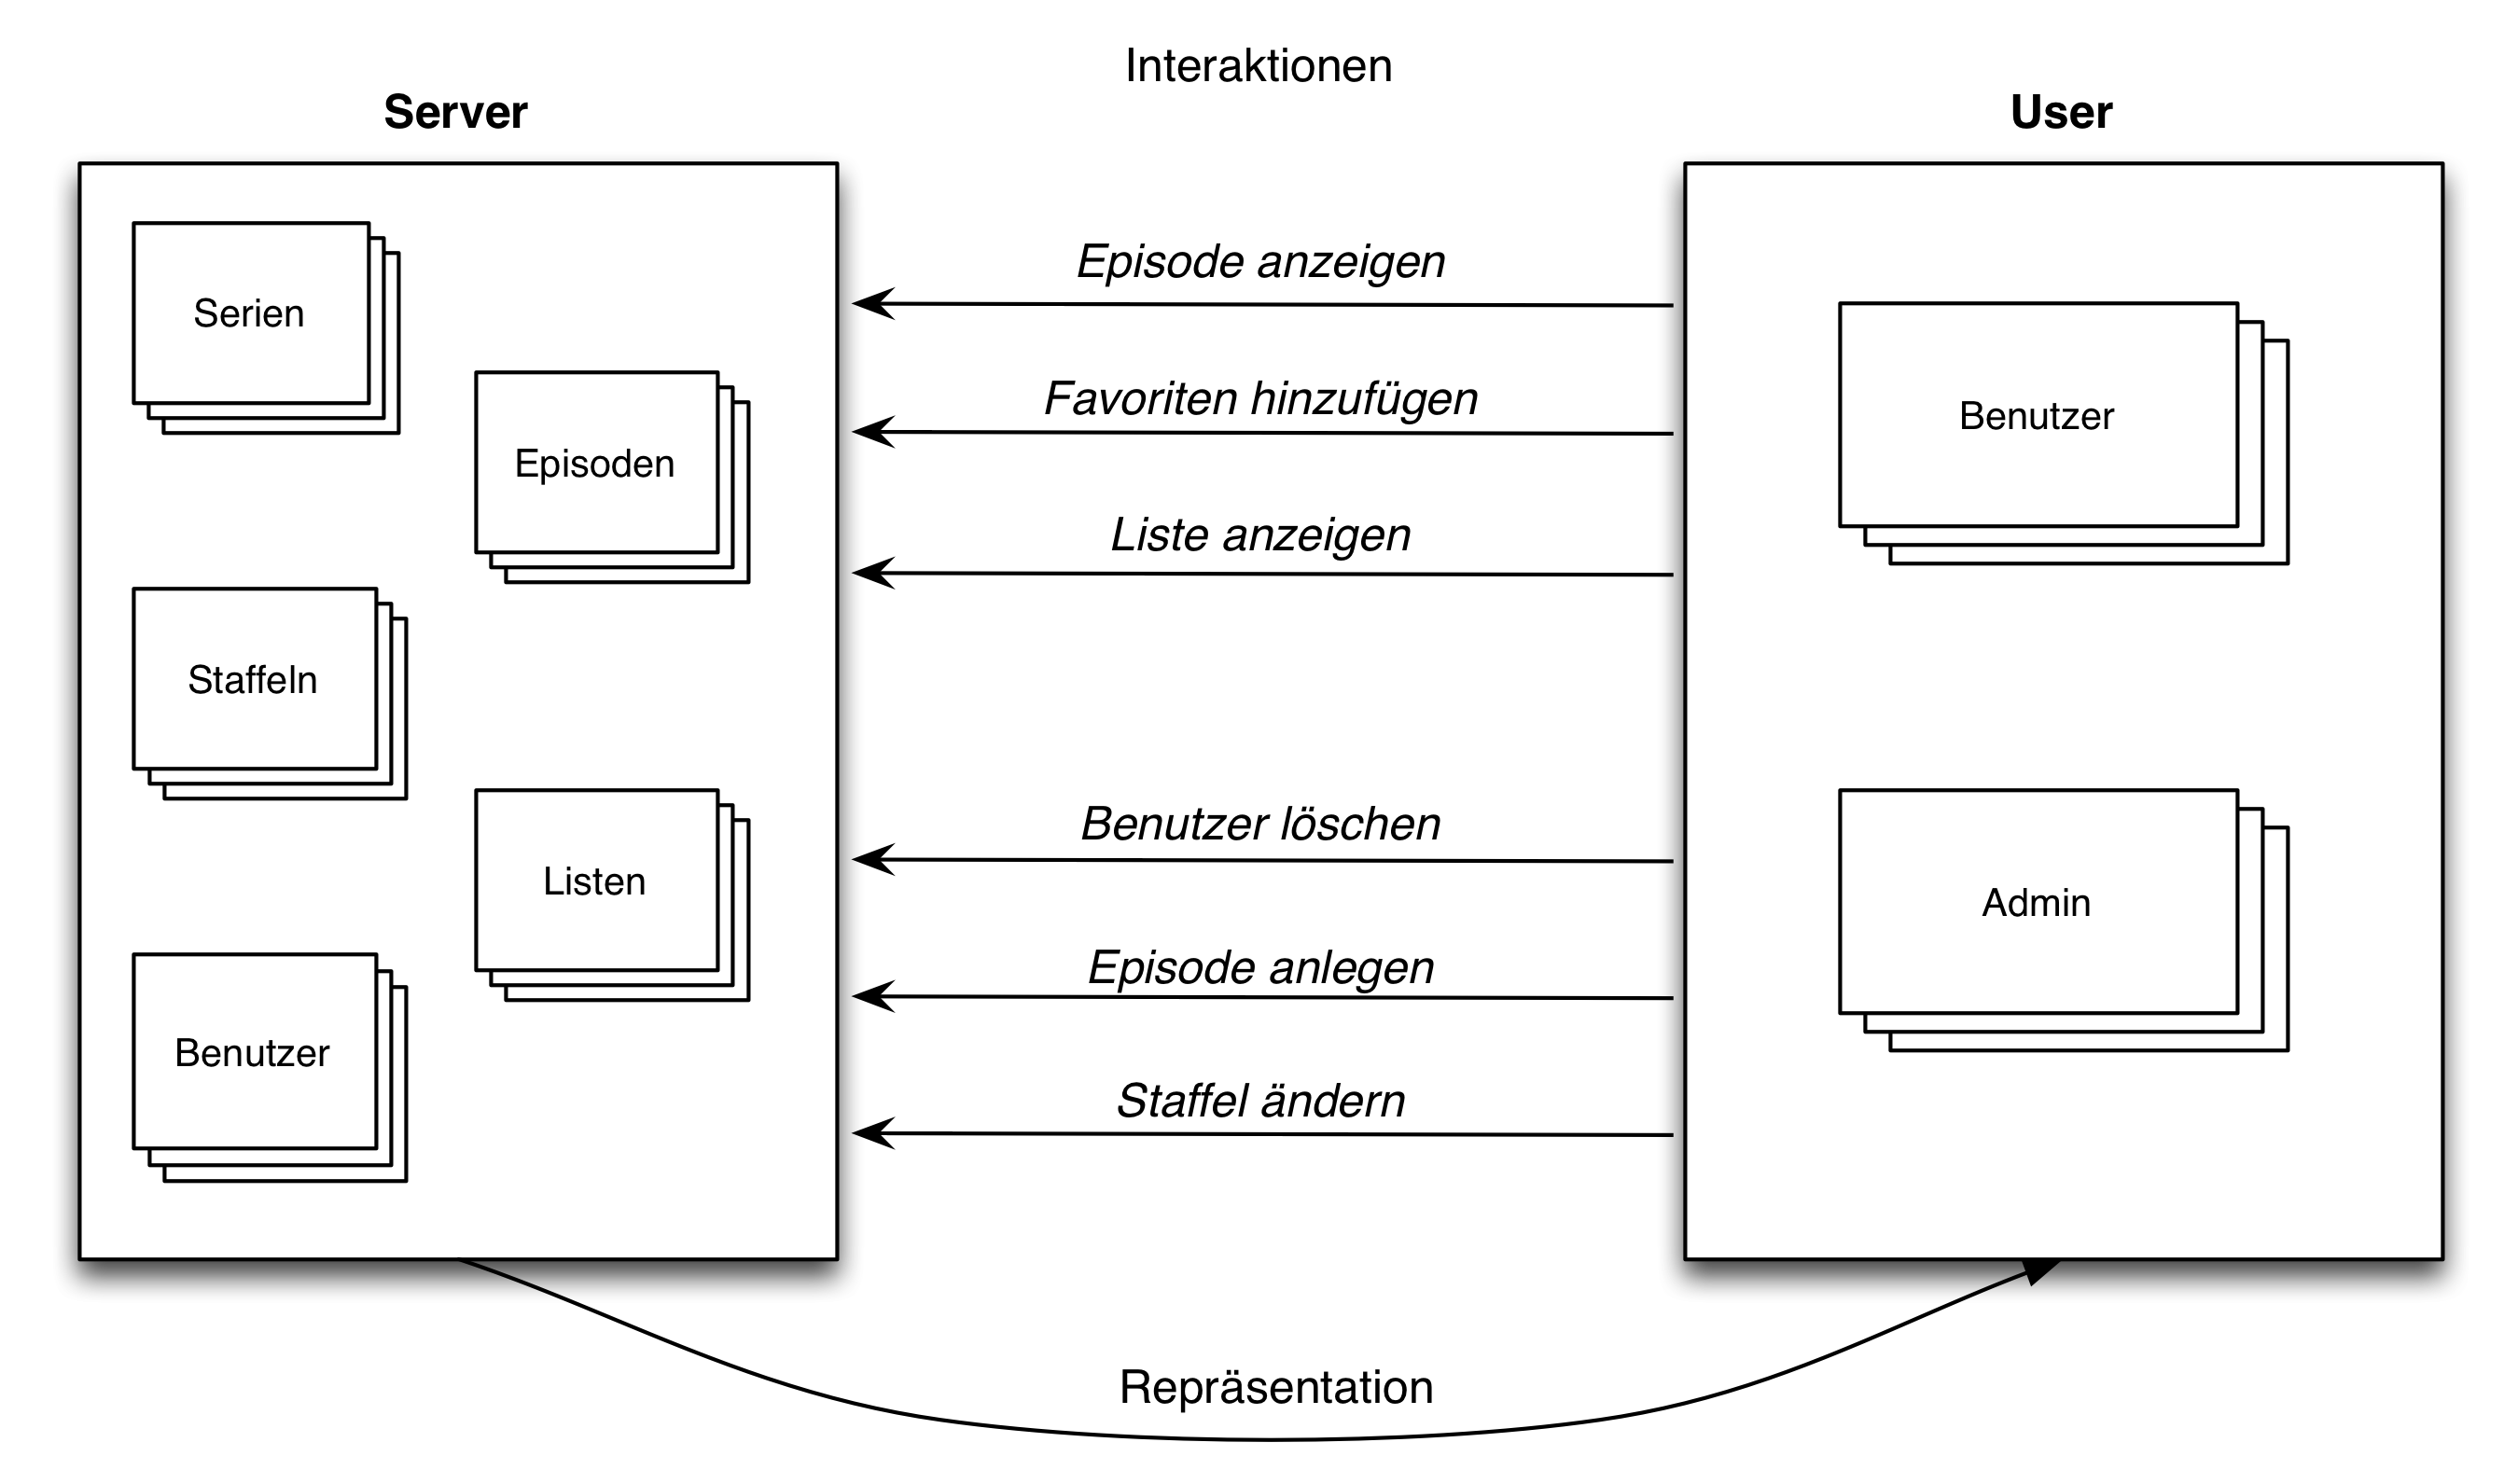
\includegraphics[width=1\textwidth]{images/kommunikationsablaeufe.png}
\caption{Synchrone Kommunikationsabläufe}
\label{kommunikationsablaeufe}
\end{figure}

Die Asynchronen Kommunikationsabläufe liefern Informationen bei bestimmten Events vom Server an die entsprechenden User als Empfänger. Dieser Ansatz wird mit Hilfe von XMPP realisiert werden und ist im Kapitel X.X genauer dargelegt. 

\begin{figure}[H]
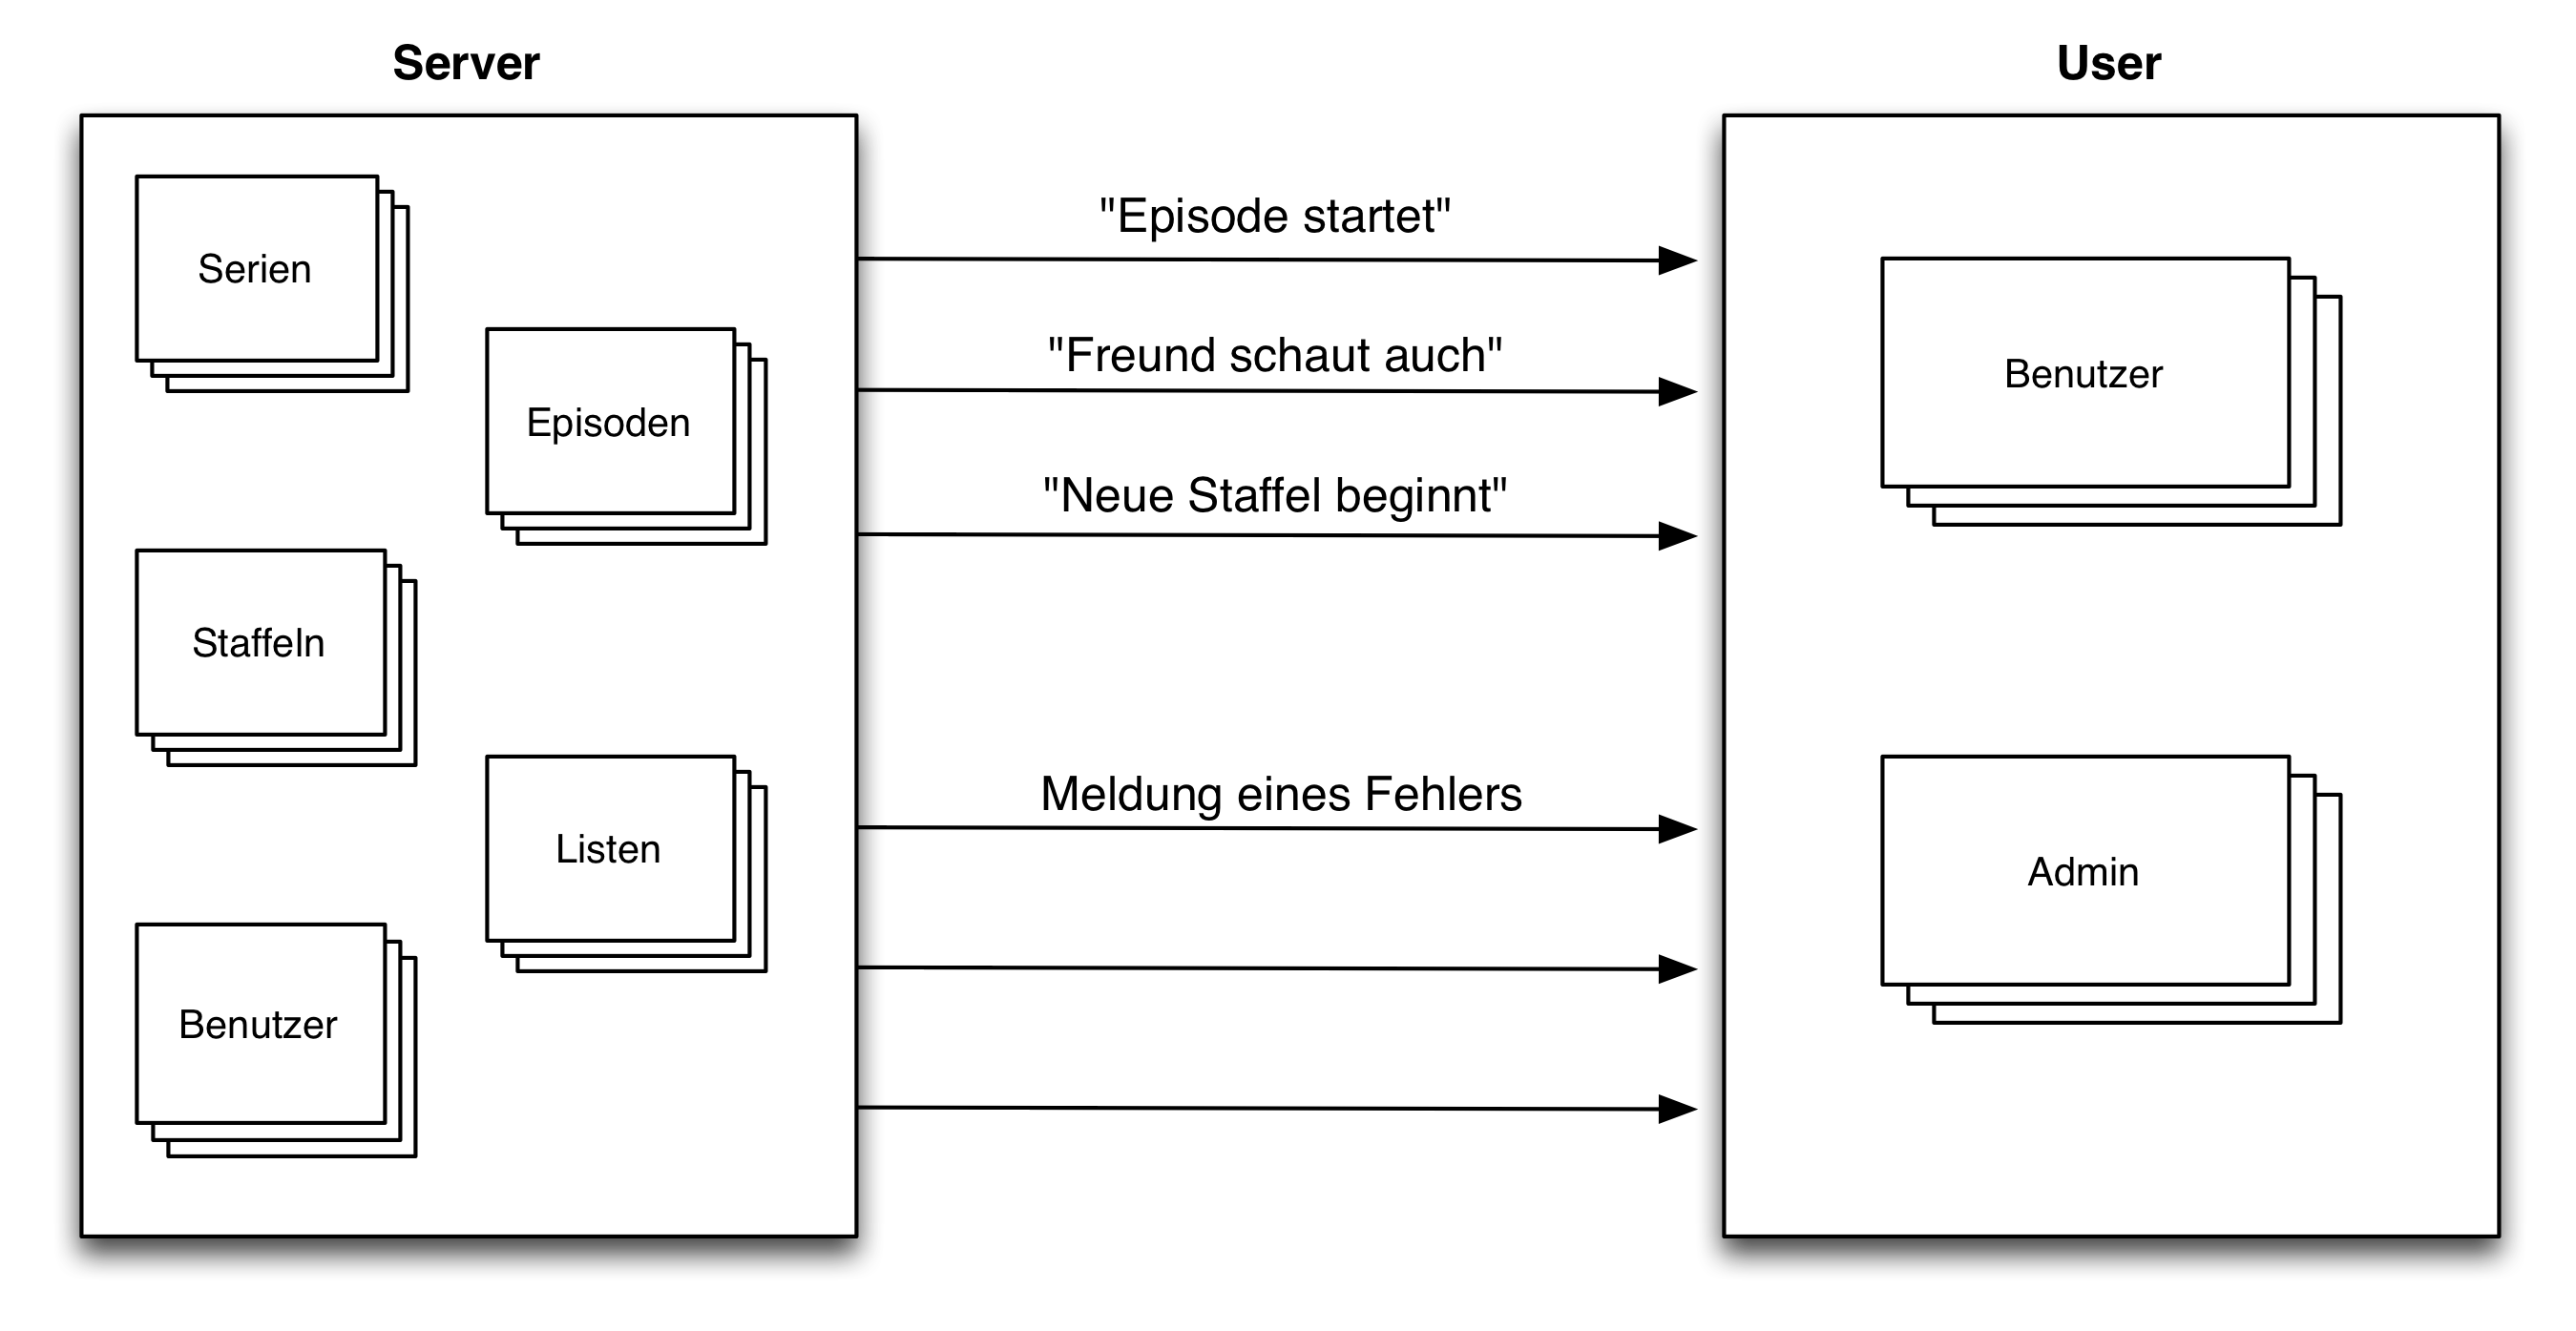
\includegraphics[width=1\textwidth]{images/kommunikationsablaeufeAsynchron.png}
\caption{Asynchrone Kommunikationsabläufe}
\label{kommunikationsablaeufeAsynchron}
\end{figure}


\newpage

\section{Entwicklung des Projektes}

\subsection{Projektbezogenes XML Schema / Schemata}
\subsubsection{Vorüberlegungen}
Der erste Meilenstein befasst sich mit der Repräsentation von Daten in XML.

Damit bei der Verwendung der XML Dateien bei der späteren Verarbeitung mit JAXB keine Probleme auftreten,
ist es notwendig eine Validierung der Dateien durch Definition zugehöriger XML Schemas durchzuführen.
Vorteil bei der Verwendung eines Schemas ist, neben der Kontrolle auf Wohlgeformtheit und der Verwendung
definierter Datentypen und Strukturen, auch das festlegen von Restriktionen.

Hinsichtlich des zugrunde liegenden Konzeptes und den benötigten Informationen, gibt es viele Elemente
innerhalb der Dateien, die nur mit Strings realisiert werden können. Das Problem bei freier Definition
besteht darin, dass die Datensätze sehr fehleranfällig sind, wenn es um die Benutzung durch Menschen geht.
Rechtschreibfehler beim Namen des Landes, des Fernsehsenders oder des Genres, würden für den Benutzer der 
Anwendung noch kein Problem darstellen, da er vermutlich deuten könnte was gemeint ist.
Für die Umsetzung ist es aber von Vorteil, die Datensätze möglichst konsistent zu halten.

Das System des Serientrackers beruht darauf, die Verwaltung von Serien anhand von Listen zu ermöglichen. Wie bereits in der Besprechung der Umsetzung erwähnt, wird anhand dieser Informationen auch die asynchrone Datenübertragung realisiert. 
Das Abonnieren von Informationen zu laufenden Serien des Genre Action, greift bei Benachrichtigung auf
Datensätze zu, die diesem Elementwert unter dieser eindeutigen Zeichenfolge zugeordnet sind. Formulierungsfehler
wie Aktion, die von einer einheitlichen Schreibweise abweichen, führen dementsprechend zu Komplikationen, weil sie die Konsistenz der Informationssätze beschädigen. \\\\

Hinsichtlich des Themas Serien, führten die Vorüberlegungen zu dem Entschluss, dass folgende Objekttypen innerhalb des Serientrackers von interesse sind und wiederkehrende Elemente darstellen:

\textbf{Serie} \\
Eines der wichtigsten Elemente, dass alle Informationen beinhaltet, die für den Benutzer von bedeutung sind, ist die Serie. 
Eine Serie besitzt allgemeine Informationen wie Name, eine Beschreibung, der Sender indem sie ausgestrahlt wird oder das Produktionsland.
Im realen Kontext wird eine Serie zudem in Seasons (Staffeln) ausgestrahlt, die jeweils eine bestimmte Anzahl von Episoden enthalten.

\textbf{Season} \\
Bestandteil einer Serie, von der es im Laufe der Jahre immer neue Objekte gibt und die nach einer gewissen Anzahl an Episoden als abgeschlossen gelten.

\textbf{Episode} \\
Ein Kernelement des Systems, dass ein wichtigen Typ für die asynchrone Kommunikation darstellt. Durch das Abonnieren von Genres oder Serien, wird die Benachrichtigung in Bezug auf eine einzelne Episode ausgelöst, die sich durch ihr jeweiliges Austrahlungsdatum und -zeitpunkt kennzeichnet. 
Zudem kann der Inhalt der Episode von Interesse sein.

\textbf{User} \\
Neben den Serieninformation, gibt es die Benutzer des Serientrackers, die sich anmelden und durch Listen die Dienste des Serientrackers abonnieren.
Allgemein werden hierbei personenbezogene Daten wie Username und echter Name erwartet, so wie Zusatzinformationen, die für andere Benutzer von Interesse sein könnten und die Person hinter dem Profil genauer beschreiben. Beispiele wären das Alter, ein Profilbild, Wohnort oder eine kurze Beschreibung.

\textbf{Liste} \\
Die Liste kann als Sammlung mehrerer Serien zu einem bestimmten Thema aufgefasst werden. Hierbei gibt zum einen Listentypen die definitiv vorhanden sein müssen, wie beispielsweise Genrelisten oder die Favoritenliste eines Benutzers. Diese erfasst die Serien, zu denen der Eigentümer Benachrichtigungen erhalten will. Zum anderen besteht aber auch die Möglichkeit, dass der Benutzer sich Listen anlegt, die seinen individuellen Wünschen entsprechen.

\textbf{Message} \\
Als zusätzlicher Typ, der jedoch erst in der asynchronen Kommunikation verwendung finden wird, wurde die Message identifiziert. Hierbei handelt es sich um eine bestimmte Nachricht, die den entsprechenden Usern bei eintreten eines Eventes zugeschickt wird und ein eintretendes Ereignis meldet.



\newpage

\subsubsection{Umsetzung}

Nach der theoretischen Planung fand die Realisierung der XML Schematas statt.
Dabei wurde für jeden der zuvor identifizierten Obertypen ein eigenes Schema definiert und die einzelnen Elemente/Attribute mit Datentypen und Restriktionen belegt. Die Aufteilung der einzelnen Typen auf ein seperates Schema, fand mit den Gedanken statt, die Struktur der Daten möglichst einfach und lesbar zu halten. Eine Serie die mehrere Staffeln enthält, die wiederrum jeweils eine Menge von Episoden auffassen, würde ein sehr komplexes Element definieren, dass während der Entwicklung schnell zu unübersichtlich werden kann.

Da die Daten einer Episode, inhaltlich jedoch weiterhin davon abhängen, von welcher Serie diese ist und in welcher Staffel sie vorkam, wird eine Referenzierung mit Hilfe von global eindeutigen IDs eingeführt. Jede Serie, User, Season, Episode, Message und Liste wird mit einer einzigartigen Folge von Zeichen beschrieben, über diese es möglich ist auf gewünschte Informationen zuzugreifen und entsprechende Elemente auszulesen.

Dieses Prinzip lässt sich am Beispiel des XML Schemas einer Episode veranschaulichen. Hierbei handelt es sich um einen Codeauszug, der die gesamte Struktur einer Episode vorgibt:
\begin{lstlisting}[label=xsd-definition,caption= Definition des complexElement Episode mit Elementen und Attributen]
  <xs:element name="episode">
    <xs:complexType>
      <xs:choice minOccurs="0">
        <xs:sequence>
          <xs:element ref="episodeNumber"/>
          <xs:element ref="title"/>
          <xs:element ref="overview"/>
          <xs:element ref="airdate"/>
          <xs:element ref="images"/>
        </xs:sequence>
      </xs:choice>

      <xs:attribute ref="serieID" use="required"/>
      <xs:attribute ref="seasonID" use="required"/>
      <xs:attribute ref="episodeID" use="required"/>
    </xs:complexType>
  </xs:element>
\end{lstlisting}

Eine Episode bekommt damit eine eindeutige \textbf{episodeID} zugeordnet und ist damit gesehen unter allen Episoden eindeutig identifiziert. Zudem erhält jede Episode auch die Referenz der serienID und seasonID als Attribute, um Verweise und Zuordnungen zu realisieren. Da sich jedes Objekt demnach durch eine Kennung repräsentiert, reicht bei anlegen von Listen und Containern ein einfacher Verweis auf entsprechendes Element, wodurch Datenredundanz bei mehreren Schematas verhindert wird, die inhaltlich voneinander abhängen. Innerhalb der XML Datei einer Serie, reicht somit der Verweis auf die einzelnen Seasons über ihre ID, ohne dass deren Inhalte mehrfach abgespeichert werden müssen. 
Dieser Redudanzverlust wäre auch realisierbar gewesen, wäre eine Season und Episode direkt innerhalb des Serieschemas gespeichert worden. Damit hätte eine Referenz auf die Serie genügt und auf eine Episode könnte mit einer Abfrage der Seasonnummer und Episodennummer getätigt werden. Der Entschluss zur Aufteilung der Schematas führte jedoch zwangsläufig zu dieser Entscheidung, wobei die Folge daraus auch komfortable Vorzüge in der Flexibilität der einzelnen Elemente mit sich bringt.


\parskip 12pt
\parindent 0pt
Um die Struktur des gesamten Serien Elements zu ermöglichen und vorhandene IDs global nutzen zu können, wird jedes Schema über eine Masterdatei in die einzelnen XML Schemas inkludiert, um bereits definierte Elemente und Attribute wiederverwendbar zu machen und die Datenmenge zu reduzieren.

\begin{lstlisting}[label=xsd-definition,caption= Auszug aus der Masterinklude Serientracker.xsd]
<!-- Dieses Schema inkludiert alle zu verwendenen Schemata-->

<xs:schema xmlns:xs="http://www.w3.org/2001/XMLSchema">

  <xs:include schemaLocation="Series.xsd"/>
  <xs:include schemaLocation="Serie.xsd"/>
  <xs:include schemaLocation="Seasons.xsd"/>
  <xs:include schemaLocation="Season.xsd"/>
  <xs:include schemaLocation="Episodes.xsd"/>
  <xs:include schemaLocation="Episode.xsd"/>

  <xs:include schemaLocation="Lists.xsd"/>
  <xs:include schemaLocation="List.xsd"/>
  <xs:include schemaLocation="Users.xsd"/>
  <xs:include schemaLocation="User.xsd"/>
  <xs:include schemaLocation="Message.xsd"/>


  <!-- Globale Elemente -->
\end{lstlisting}

Neben dem Include der eunzelnen Schematas, werden auch vereinzelte Elemente darin definiert, die innerhalb der einzelnen Schematas wiederholt Verwendung finden. Hierbei vor allem die einzelnen ID Attribute. \\

Während der Entwicklung dieser Variante, gab es anfängliche Schwierigkeiten innerhalb der Umsetzung. Der Verweis innerhalb eines XML Schemas auf ein Anderes und die entsprechende Verwendung der Elemente und Attribute, führte zu Komplikationen innerhalb der Deklarationen. Auch eine Definition eines einheitlichen Namespaces führte zu keiner Lösung. Im zweiten Ansatz folgte dann die direkte Auseinandersetzung zwischen den Optionen Include und Import, wobei die letztendliche Wahl auf die Inkludierung fiel. Ein Import erlaubt den Verweis auf unterschiedliche Namespaces, wobei ein Include auf einen einheitlichen Namespace verweist und bei nichtbestehen, den des Oberschemas übernimmt.
Da Namespaces in der Regel dazu dienen, Elementen und Attributen einen gewissen Namensraum zu gewährleisten, der bei gängigen Bezeichnungen wie \textit{Name} zu Konflikten führen kann, ist die Definition bei größeren Projekten durchaus zu empfehlen. Ob dabei ein Einzelner oder Mehrere angelegt werden sollten, ist eventuell auch abhängig von der gesamten Struktur des Schemas. Da im Rahmen dieses Projektes jedoch mit relativ geringem Datenumfang gearbeitet wird und mit keiner Komplikation der Bezeichnungen zu rechnen ist, wurde auf eine genaue targetNamespace Definition verzichtet. Auch wenn bestimmte Elementbezeichnungen innerhalb eines \textit{http://Serientracker.de} Namensraum denkbar gewesen wäre. Letztendlich spielt dieser Aspekt für die Umsetzung innerhalb des Projektes jedoch keine tragenden Rolle. Daher wurde auf die Definition verzichtet und die entsprechende Include Variante verwendet. 


Ein weiterer Punkt der in der Entwicklungsphase von Bedeutung war, war die Frage danach, wie die Daten innerhalb des lokalen Speichers abgelegt werden.
Durch die Definition einzelner Schematas erhält jedes Objekt dieses Typs auch eine eigene XML Datei. Im späteren Verlauf könnten sich daraus aber Probleme beim gezielten Zugriff entwicklen, denen frühzeitig Abhilfe geschaffen werden sollte.
Aus diesem Grund wurde eine weitere Gruppe von Elementen innerhalb XML angelegt, die Containerklassen. 
Für jeden Elementtyp, der als eigene Entität angelegt wird, wurde eine Containerklasse definiert, innerhalb derer beliebig viele Objekte eines bestimmten Typs aufgenommen werden können. Dieses Objekt dient in der letztendlichen Verwaltung als Sammlung aller Elemente.

Folgendes Beispiel veranschaulicht den Ansatz und wurde in dieser Form für jeden Elementtyp angelegt:


\begin{lstlisting}[label=xsd-definition,caption= Auszug aus der Series.xsd Definition]
<!-- Element das alle Serien aufnimmt -->
  <xs:element name="series">
    <xs:complexType>
      <xs:sequence>
        <xs:element ref="serie" minOccurs="0" maxOccurs="unbounded"/>
      </xs:sequence>
    </xs:complexType>
  </xs:element>
\end{lstlisting}


Um die vorhandenen Daten semantisch sinnvoll und reichhaltig anzulegen, wurde bei der Entwicklung der XML Schematas darauf geachtet, diesen Anspruch 
durch die verschiedenen Datentypen, Restriktionen und Benutzungstypen zu gewährleisten.  

\newpage

\subsubsection{Datentypen}
Grundsätzlich werden innerhalb des Serientrackers Daten unterschiedlichen Typs benutzt, die entsprechend des realen Kontextes am sinnvollsten erscheinen.
Aufgrund der Komplexität, soll hierbei nicht auf jedes einzelne Element eingegangen werden, sondern nur ein Überblick darüber vermittelt werden, mit welchen Grundideen vorgegangen wurde.

Neben den einfachen Standartdatentypen wie String, Boolean, Integer, Time (...), bietet XML die Möglichkeit weitere spezifische Typen wie anyURI oder ID zu definieren.\\ 
Da innerhalb des Serientrackers viele Information lediglich in Textform sinnvoll sind, wurde für diese der Typ \textbf{String} verwendet. Beispielhaft seien hier die Titel und Beschreibungen, sowie Benutzernamen und Länder erwähnt.\\ 
Jahreszahlen, Episodenlänge und Season- und Episodennummern werden mit Zahlen als \textbf{Integer} ausgedrückt. Bestimmte Zeitangaben wie Ausstrahlungszeit, bei denen es nur um den Zeitpunkt geht, in der einfach Form \textbf{Time} und genauere Angaben, wie bei Ausstrahlungstag in Hinsicht auf die Benachrichtigung, über den \textbf{dateTime} Typ. 
Linkverweise auf Bildquellen wie bei Avatar erhielten den Typ \textbf{anyURI}.\\

Einzelne Elemente wie User und List, weisen hierbei noch eine Besonderheit auf. Wie bereits bei den Kommunikationsabläufen innerhalb des Konzepes eangesprochen, wird die Anwendung von Benutzern verwendet, die verschiedenen Rechtetypen angehören. Aus diesem Grund wird jeder User mit dem Attribute Admin gekennzeichnet, der innerhalb einer einfachen \textbf{Boolvariablen} die entsprechenden Rechte festgelegt. Ähnliches Prinzip wird bei den Listen verwenden zur Unterscheidung, ob die Sichtbarkeit für jeden Benutzer gestattet ist oder nur für den Besitzer der Liste.

\parskip 12pt
\parindent 0pt
Zur angesprochenen Referenzierung und Identifizierung einzelner Entitäten, zeichnen sie sich durch eine eindeutige ID als Attribut aus. Generell wurden die Informationen wie ID oder Rechte, die ein Objekt nicht inhaltlich sondern eher aus verwaltender Sicht genauer beschreiben, als Attribute definiert. Inhaltliche Informationen die Bestandeteil des Objektes sind, werden hingegen als Elemente angelegt.

Für den Datentyp einer solchen ID, wurde ein eigenes Element folgendermaßen definiert:
\begin{lstlisting}[label=xsd-definition,caption= Definition der globalen ID's]
  <xs:simpleType name="idType">
    <xs:restriction base="xs:string">
      <xs:pattern value="|(ss|sn|ep|us|ls|me)_[0-9a-z]{8}"/> 
    </xs:restriction>
  </xs:simpleType>
\end{lstlisting}

Am Anfang der Zeichenketten steht ein Kürzel, dass den jeweiligen Typ angibt. SN steht dabei für Season, EP für Episode und ähnliches. Danach folgt ein optisches Trennzeichen, gefolgt von einer beliebigen Characterfolge aus 8 gemischten Zeichen mit Zahlen und Buchstaben. Eine Serie erhält damit eine Zuordnung der Form \textit{ss\_0a1b2c3d}.



\subsubsection{Restriktionen}
Damit die Informationen innerhalb der XML Datein inhaltlich sinnvoll sind und während der Verarbeitung keine weiteren Probleme entstehen (zum Beispiel durch unterschiedliche Schreibweisen), wurden für einige Elemente Restriktionen definiert.
Dabei ist das Ziel, die Fehleranfälligkeit zu reduzieren und im Kontext logische Informationen zu gewährleisten. Vorhandene Restriktionen, also Einschränkungen/Bedingungen, die für einzelne Elemente getroffen wurden sind im folgenden mit einer kurzen Begründung aufgeführt. Häufig treten diese in Form von Längenbegrenzungen bei Texten auf oder als Grenzbereichen bei Zahlen auf.\\
Weitere Elemente kennzeichnen sich entsprechend dadurch, dass der Inhalt auf eine bestimmte Auswahl an Möglichkeiten eingeschränkt wurde. Beim Konzipieren dieser Grenzen und Auswahlmöglichkeiten, ist es nicht möglich die perfekte Variante zu erzielen, sondern eine Auswahl von Optionen zu treffen, die im Kontext als zuverlässig und praktikabel erscheinen. Manche Begrenzugnen wie Anzahl an Episoden einer Staffel oder Episodenlaufzeit, wurden in Bezug auf die Realität getroffen und angelehnt an gängige Formen. Prinzipiell wären hierbei  alternative Auswahlmöglichkeiten und Varianten denkbar, wie beispielsweise die freie Definition des Genres oder des TV Senders als einfacher String. Hierbei hat der verwaltende Admin dann die Option den Inhalt frei zu bestimmen. Letztendlich wurde jedoch der eigentliche Nutzen abgewägt, sodass für den Serientracker folgende Restriktionen definiert wurden:

\begin{table}[H]
\caption{Allgemeine Restriktionen}


\begin{tabular}{l l l}
\\ [-0.5ex]

\hline\hline
\\ [-0.5ex]
Element/Attirbut & Restriktion & Begründung
\\ [1.5ex]
\hline
\\ [-0.5ex]
Overview (global) & Stringlänge 10 < und < 500 & allgemeinen Informationen,\\[1ex]
&&kurze Inhaltsangabe\\[3ex]
Title (global) & Stringlänge 1 < und < 80 & gängige Titellänge\\[3ex]
Name (list) & Stringlänge 2 < und < 80 & treffende Bezeichnung,\\[1ex] 
&&Name keine Beschreibung \\[3ex] 
Public (list) & Boolean True und False & feste Zustände \\[3ex] 
Episodenumber (episode) & Anzahl < 26 & sinnvolle maximale Episodenanzahl\\[3ex] 
Seasonnumber (seasons) & Anzahl < 41 & sinnvolle Begrenzung, \\[1ex]
&&Freiraum für Langzeitserien \\[2ex] 

\hline
\end{tabular}
\label{tab:restriktionenderxsd}
\end{table}


\begin{table}[H]
\caption{Restriktionen des User Schemas}
\centering

\begin{tabular}{l l l}
\\ [-0.5ex]

\hline\hline
\\ [-0.5ex]
Element & Restriktion & Begründung
\\ [1.5ex]
\hline
\\ [-0.5ex]
Username & Stringlänge 2 < und < 30 & sinnvolle Namenlänge,\\[1ex]
&& verhindert Text \\[3ex]

Lastname & Stringlänge 1 < und < 40 & gängige Nachnamenlänge, \\[1ex]
&&eventuell Doppelnamen,\\[1ex]
&&verhindert Text \\[3ex]

Firstname & Stringlänge 1 < und < 50 & gängige Vornamenlänge, \\[1ex]
&&Mehrfachnahmen \\[3ex]

Gender & Auswahl zwischen Male und Female & logische Auswahl, \\[1ex]
&&Vorgabe verhindert Schreibfehler\\[3ex]

Age & älter als 13 und jünger als 121 & Mindestalter zur Nutzung, \\[1ex]
&&logische Obergrenze \\[3ex]

Location & Stringlänge < 40 & Stadtname, Land etc. \\[1ex]
&&Eingabe ist keine Adresse\\[1ex]
&&und lässt sich in Kürze ausdrücken\\[3ex]

About & Stringlänge < 200 & optionale Kurzbeschreibung,\\[1ex]
&&nach oben begrenzt, \\[1ex]
&&zu viele Informationen nicht \\[1ex]
&&unbedingt von Interesse  \\[3ex]

Admin & Boolean ob True or False & Rechtevergabe nach Status,\\[1ex] 
&&Auswahl nur in 2 Zuständen möglich\\[2ex]

\hline
\end{tabular}
\label{tab:restriktionenderxsd}
\end{table}


\begin{table}[H]
\caption{Restriktionen des Serie Schemas}


\begin{tabular}{l l l}
\\ [-0.5ex]

\hline\hline
\\ [-0.5ex]
Element & Restriktion & Begründung
\\ [1.5ex]
\hline
\\ [-0.5ex]
Year & Jahreszahl 1900 < und < 2015 & Jahreszeiten außerhalb\\[1ex]
&&unrelevant \\[3ex]

Country & Auswahlmöglichkeit Ländern & Eingabefehler verhindern\\[3ex]
Episoderuntime & Auswahl zwischen gängigen Episodenlängen& Serie hat feste Episodenlänge\\[3ex]
Network & Auswahl bekannter Sender & unrelevante Sender entfallen,\\[3ex]
&&Eingabefehler verhindern\\[3ex]

Airday & Auswahl des Tagnamen & Eingabefehler verhindern\\[3ex]
Genre & Auswahl definierter Genres & einheitliche Schreibweise,\\[1ex]
&&Eingabefehler verhindern,\\[1ex]
&& sinnvolle Genre\\[2ex]

\hline
\end{tabular}
\label{tab:restriktionenderxsd}
\end{table}



\subsubsection{Beispieldaten}

Bereits während der Entwicklung der XML Schemas, wurden parallel XML Dateien mit entsprechenden Beispieldaten definiert. Durch den entsprechenden Validierungstest bietet sich zum einen die Möglichkeit entsprechenden Definitionen auf Korrektheit zu prüfen und zum anderen XML Typen zu entwickeln, die möglichst praxistaugliche Elemente und Attribute aufweisen. Zu jedem XML Schema wurde daher mindestens eine Beispieldatei erzeugt und die entsprechende Referenzierung untereinander getest. Speziell im Containerelemente Series wurde deutlich, wie flexibel die Datensicherung mit globalen IDs sein kann. Zum einen reicht das Einbinden eines Objekts in der simplen Form <serie serieID="ss\_6127hdja"/>, zum anderen kann auch die gesamte Struktur einer Serie inklusive Informationen über Season und die einzelnen Episoden eingebunden werden. \\

Für die entsprechende Nutzung in der weiteren Entwicklung, wurden zudem korrekte Beispieldatensätze von Serien angelegt. Diese Repräsentieren von der obersten Ebene der allgemeinen Serieninformationen bis hin zur niedrigsten Ebene der einzelnen Episodeninformation vollständige Datensätze, wie sie in einem komplexen System dieser Form angelegt werden müssten. Aufgrund von Testzwecken, wurde sich jedoch auf wenige Beispielserien beschränkt. Zudem wurden entsprechende Daten innerhalb der Series.xml definiert und nicht in die entsprechenden Typen aufgeteilt. Diese Variante hatte zum Vorteil, dass die Informationen einer Serie (für Menschen) übersichtlich strukturiert und lesbarer waren, als wenn jede Beispielepisode per Hand in einzelne XML Files getrennt worden wäre.
Aufgrund der Vielzahl von Informationen zeigte, sich aber bereits bei wenigen Daten der Nachteil, dass die Datei sehr komplex wurde. Darüber hinaus weist diese Variante auch die Schwäche beim möglichen Datenverlust auf. Sollte in diesem Fall das sammelnde Element verloren gehen, so wäre der Datenverlust größer gegenüber den seperaten Absicherungen in einzelne Files.


\parskip 12pt
\parindent 0pt
In der Konzeptvorstellung wurde bereits von der möglichen Einbindung einer Freundefunktion gesprochen. Die Umsetzung dieses Thema würde noch eine Änderung der XML Schematas der User mit sich ziehen. Ähnlich wie für die Abonnements von Serien, könnte man innerhalb des User Schemas ein komplexes Element \textit{Friends} einbauen, dass beliebig viele User aufnimmt. Dabei könnten normale Objekte des bereits vorhandenen Userschemas eingebunden werden und eine Liste aller Freunde bilden.\\ Um die entsprechende Kommunikation zwischen den einzelnen Freunden zu gewährleisten und Meldungen wie Empfehlungen oder Benachrichtigungen zu verschicken, muss weiterhin das Message Schema erweitert oder alternativ ein neues Schema der \textit{Friendmessage} eingeführt werden. Eine seperate Trennung beider Nachrichtenarten wäre in sofern sinnvoll, als das diese in der Funktionalität und Definition unterschiedliche Anwendungen haben. Die bisherigen Nachrichten werden von der Serverseite aus an User geschickt und beinhalten statische Nachrichten. Auch Empfehlungen könnte man mit festen Standartnachrichten wie \textit{X empfiehlt dir Serie Y} umsetzen, jedoch wäre hierbei innerhalb eines realen Kontext wahrscheinlich eine persönlichere Komponente wie Userkommentare mit enthalten.


\parskip 12pt
\parindent 0pt
Sofern dieser Aspekt umgesetzt wird, müsste man hierbei die entsprechenden Varianten abwägen und dabei mögliche Szenarien konzeptionell durchspielen, um eine passende Einbindung hinsichtlich der Funktionalität zu finden.\\
Nach der Auseinandersetzung mit den vorhandenen Daten und entsprechender Definition der XML Schemas, folgt im nächsten Schritt die Entwicklung der synchronen Kommunikationskomponenten.


\newpage

\subsection{Ressourcen und die Semantik der HTTP-Operationen}
\subsubsection{Ressourcen}

Als Vorbereitung für die Umsetzung der synchronen Kommunikationsvorgänge, steht die theoretische Auseinandersetzung mit REST im Mittelpunkt.
Der erste Schwerpunkt dabei ist die Identifizierung vorhanderer Ressourcen des Serientrackers. Bereits beim Konzipieren der XML Schemas mit beispielhaften XML Datensätzen, musste überlegt werden, für welche Elemente es möglich ist Entitäten der realen Welt zu ermitteln.

Bei einer Ressource geht es, ähnlich wie bei XML Dateien, nicht darum wie die darin enthalten Informationen im letztendlichen Kontext repräsentiert werden, sondern welche Informationen diese enthalten. Entsprechende Objekte der Außenwelt werden beschrieben und wie die Wurzelelemente bei XML, stellen sie einen bestimmten Objekttyp dar. Eine identifizierte Ressource, ist eine Schnittstelle zur Außenwelt und sollte daher dem Kontext entsprechend gut durchdacht werden.
Die Auseinandersetzung mit den XML Schemas lieferte dabei einen Überblick über vorhandene Primärressourcen. Dabei handelt es sich um die Oberklassen der vorhandenen Objekttypen \textit{Serie} und \textit{User}.

Desweiteren ist es möglich vorhandene Subressourcen zu identifizieren, die sich dadurch auszeichnen, dass sie selbst Bestandteil einer Ressource sind.
Aufgrund der komplexen Struktur einer Serie, die neben den allgemeinen Informationen noch die Informationen zu mehreren Staffeln und entsprechenden Episoden enthalten, wurde früh die systematische Aufteilung festgelegt.
Da es auch innerhalb der Anwendung von Interesse sein kann, eine einfache Repräsentation der Staffelübersicht oder der Episodenübericht einer Staffel zu ermöglichen, bietet es sich gerade bei diesen Typen an, diese Objekte als eigene Ressource zu designen. Dazu kommt, dass eine Episode zum Beispiel im Kontext einer Serie am meisten Sinn macht, durchaus aber auch für sich existieren kann.Zur Ordnung der einzelnen Elemente, gibt es entsprechende Listenressourcen wie Series, Seasons, Users und Episodes, welche alle Elemente des zugehörigen Typs aufnehmen und sammeln.\\

Ein Kernelement der Anwendung wird das Benachrichtigen der Benutzer über bestimmte Ereignisse sein. Diese Abonnements lassen sich in Listen verwalten. Gerade bei einer möglichen Kategorisierung wie beispielsweise \textit{Serie mit dem Genre Drama}, wäre es durchaus interessant gewesen Listenressourcen mit entsprechenden Filtern zu definieren. Aufgrund der Vielzahl von Kategorisierungsmöglichkeit, wird dieser Schritt aber nicht über einzelne Ressourcen stattfinden, sondern innerhalb Anwendung durch die Abfrage bestimmter Elemente errzielt.
\newpage

Die theoretische Auseinandersetzung führte zu folgenden Ressourcen, wobei die angegeben URI nur den charakteristischen Abschnitt wiederspiegelt.
Da für die Umsetzung an sich, die URI eher als eine ID in Form von Zeichen steht und für die letzendliche Auswertung nicht unbedingt notwendig ist, wird auf eine Darstellung in Form mit Schema und Pfadangabe in der Übersicht verzichtet.

\begin{table}[H]
\caption{Ressourcen des Serientrackers}

\centering
\begin{tabular}{l l l}
\\ [-0.5ex]

\hline\hline
\\ [-0.5ex]
Ressource & URI & Methode
\\ [1.5ex]
\hline
\\ [-0.5ex]
Liste aller Serien & /series/ & GET, POST \\[1ex]
Einzelne Serie & /series/\{id\} & GET, PUT, DELETE\\[1ex]
Liste aller Staffeln & /seasons/ & GET, POST \\[1ex]
Einzelne Staffel & /seasons/\{id\} & GET, PUT, DELETE\\[1ex]
Liste aller Episoden & /episodes/ & GET, POST \\[1ex]
Einzelne Episode & /episodes/\{id\} & GET, PUT, DELETE\\[1ex]
Liste aller User & /users/ & GET, POST \\[1ex]
Einzelne User & /users/\{id\} & GET, PUT, DELETE\\[1ex]
Liste aller Listen & /lists/ & GET, POST\\[1ex]
Liste eines Users & /lists/\{id\} & GET, PUT, DELETE\\[1ex]
\hline
\end{tabular}
\label{tab:ressourcendesserientrackers}
\end{table}

Jedes Element, dass für die synchrone Kommunikation von Interesse ist, besitzt eine Ressource als einzelnes Element\\ 
(Form:/ressourcenname/\{id\}) und die Gesamtheit einer Liste (Form:/ressourcenname/). Bei den URI wird der Zugriff über entsprechende ID's auf die Liste deutlich und es zeigt sich eine Folge der einfachen URI. Durch die Konzipierung der Untertypen Staffel und Episode als einzelne Ressource, ist eine entsprechender Aufruf auf das bestimmte Element möglich.\\
Vorstellbar aufgrund der allgemeinen Struktur wäre auch ein Pfad der \\
Form /series/\{id\}/seasons/\{id\}/episodes/\{id\}.  Dieser setzt entsprechend vorraus, dass nicht nur die einfache Episoden ID, sondern auch die zugehörige Serien ID und Season ID bekannt ist.

\subsubsection{Semantik der HTTP-Operationen}

Nachdem die Ressourcen identifiziert sind, muss nun bestimmt werden, welche Operationen (HTTP-Methoden) unterstützt werden und welche Semantik sich dahinter verbirgt.\\
Dafür stehen die vier Methoden GET (Informationen auslesen), POST (Informationen anlegen), PUT (Informationen ändern) und DELETE (Informationen löschen) zur Verfügung. Nicht jede Ressource muss alle Methoden bereitstellen. Für das Projekt wurden die Ressourcen erneut betrachtet und die benötigten Methoden samt Semantik herausgearbeitet. Dabei entwickelte sich folgende Ergebnis:

\begin{figure}[H]
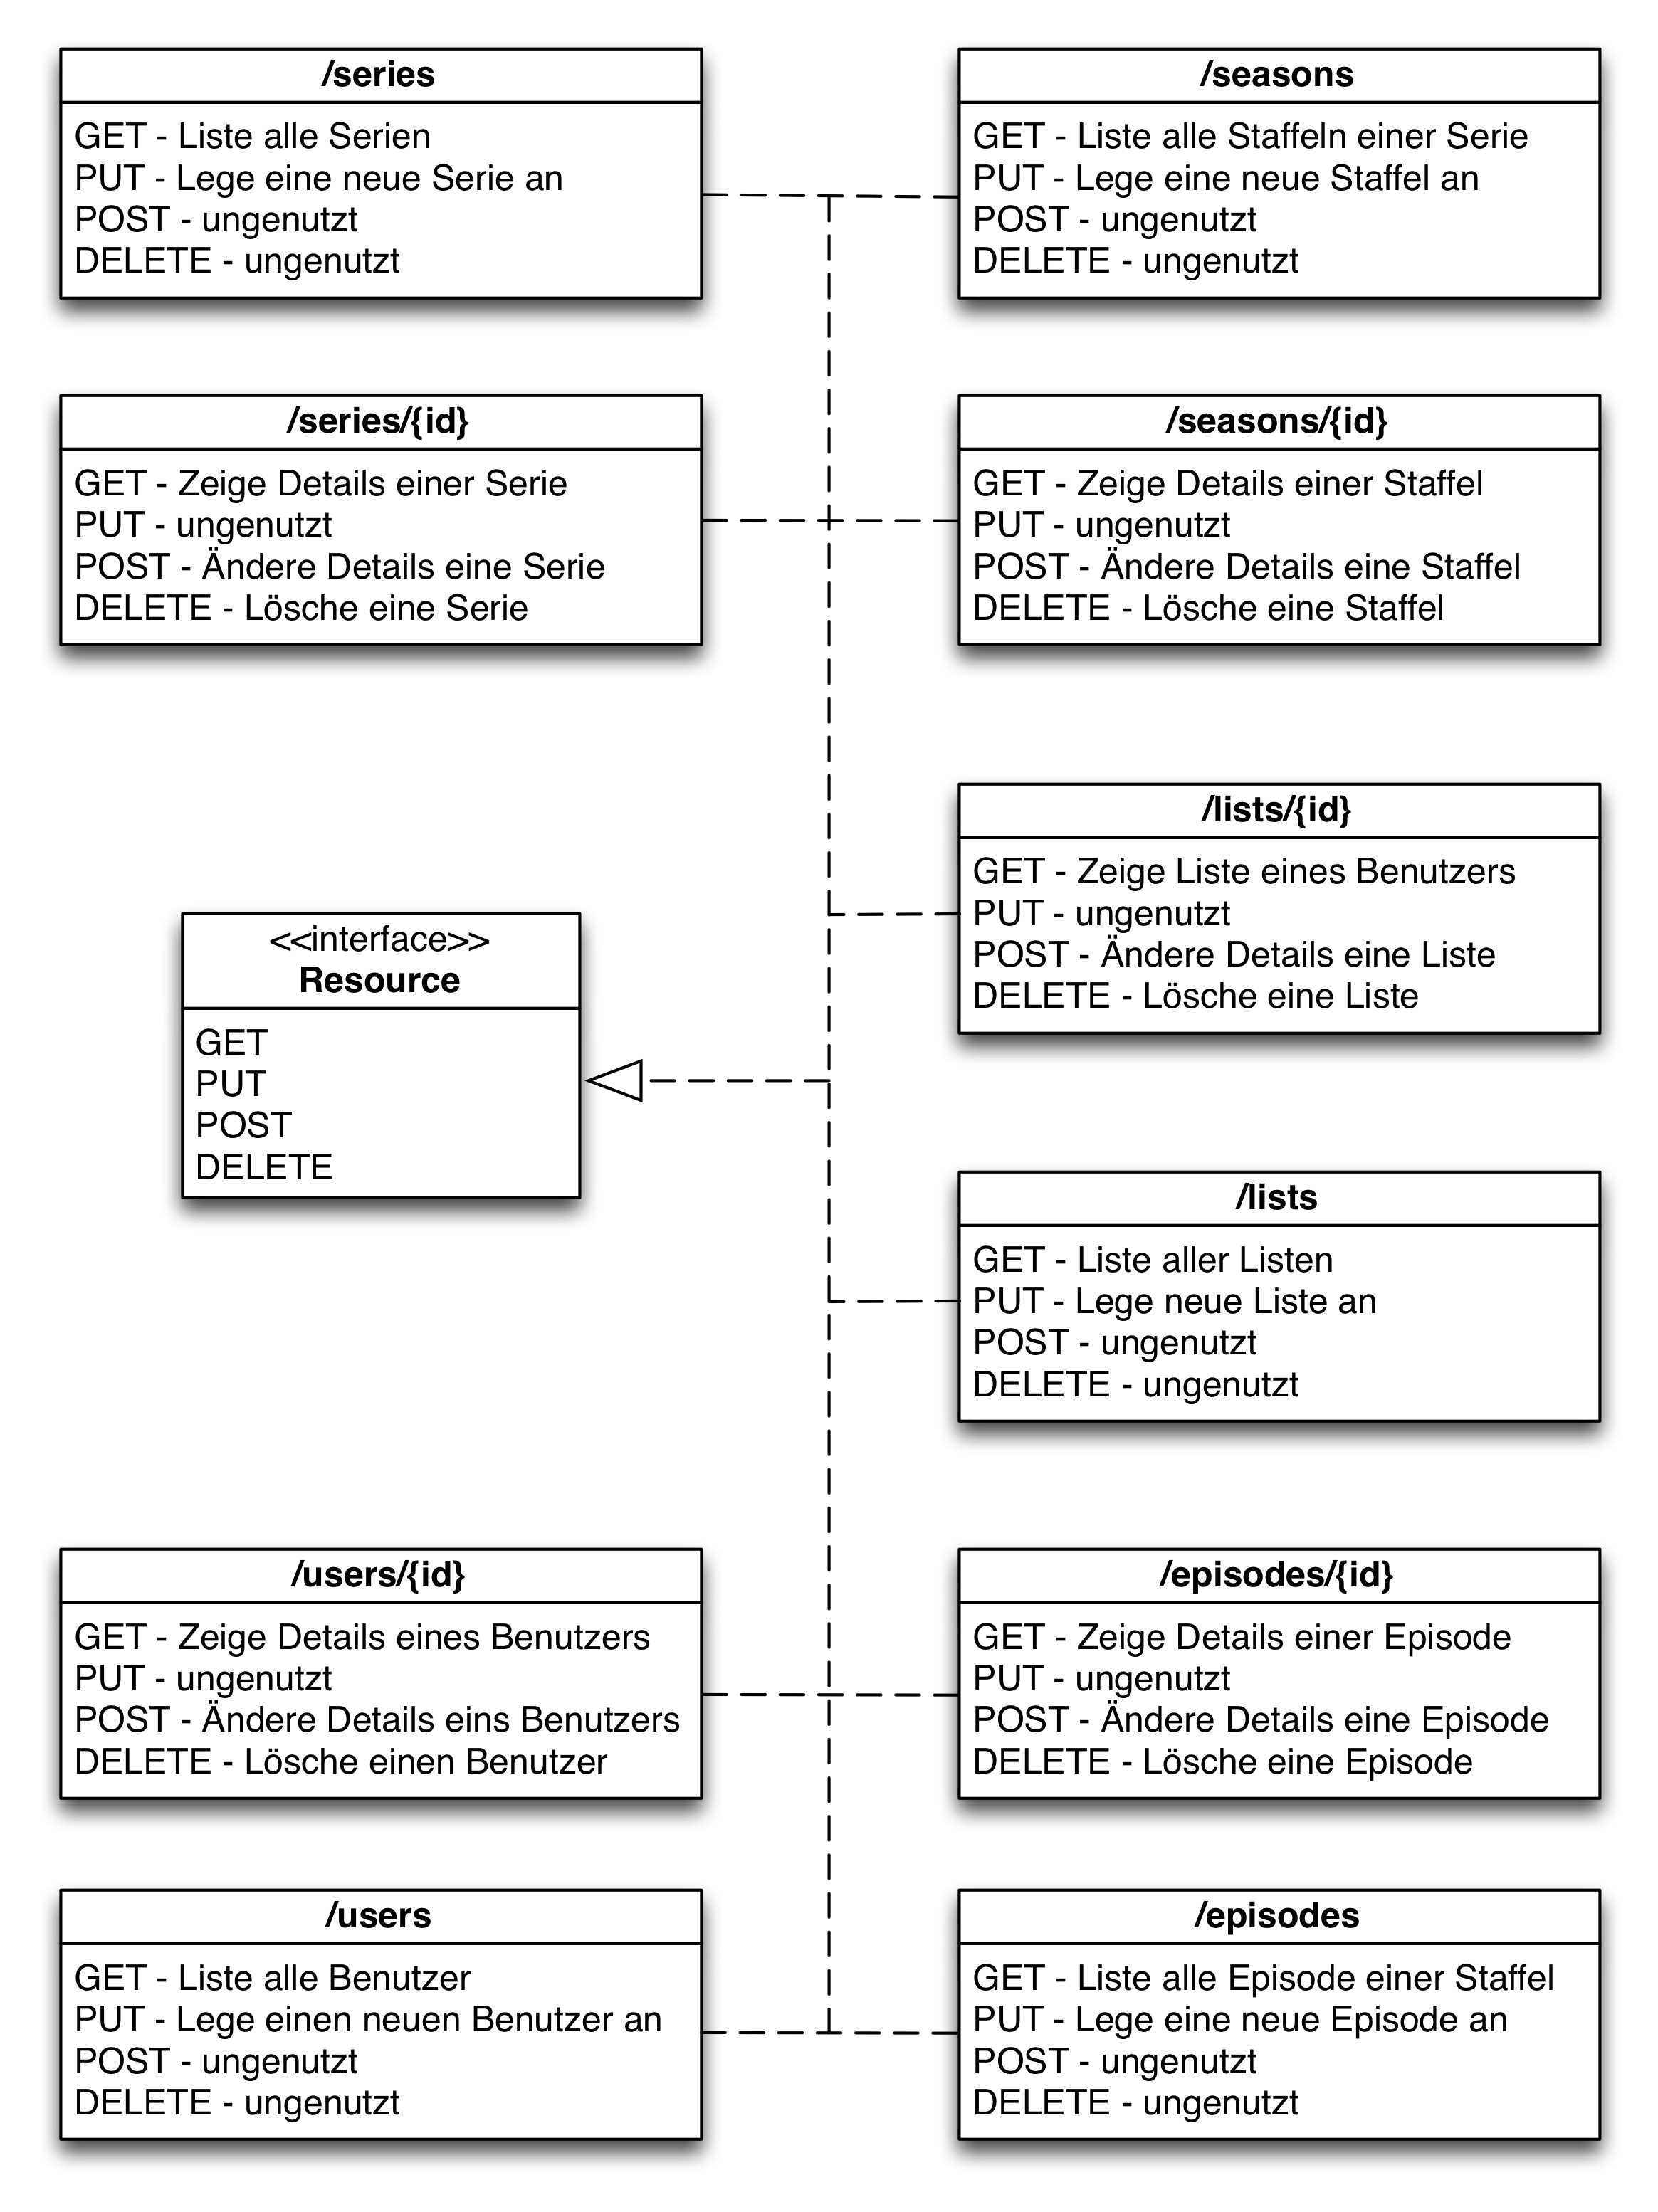
\includegraphics[width=1\textwidth]{images/bedeutunghttpmethoden.png}
\caption{Bedeutung der http Methoden}
\label{bedeutunghttpmethoden}
\end{figure}

\newpage

\subsection{RESTful Webservice}

Nach der konzeptionellen Planung der Ressourcen und HTTP - Operationen, geht es um die codebasierte Umsetzung. Definierte XML Schemas werden nach erfolgreicher Validierung in JAXB Objekte überführt, um eine Verwendung des Datenbestandes im Javaprojekt zu ermöglichen und aus den Schemadateien Java-Klassen zu erzeugen.\\
Zur Realisierung der synchronen Kommunikation wird Grizzly als Webserver der HTTP - Operationen verwendet. Zusätzlich wird zur Entwicklung des RESTful Webservices das Jersey framework implementiert, dass für JAX-RS APIs und Server als Referenzimplementierung dient. 

\subsubsection{Vorüberlegungen}
Bereits im Rahmen der Ressourcenfindung, wurde sich Gedanken darüber gemacht, wie URI zur jeweiligen Ressource gestaltet werden können, damit ein logischer Request auf gewünschte Daten stattfinden kann.

Die Repräsentation einer spezifischen Ressource wurde im vorherigen Abschnitt mittels \textbf{Path-Parameter} realisiert, das heißt, der Parameter ID war Teil der eigentlichen URI.\\
Als Alternative können allerdings auch sogenannte \textbf{Query-Parameter} zum Einsatz kommen. Diese eignen sich meistens um Ressourcen noch weiter zu verfeinern und sind in der Regel optional.

Innerhalb des Serientrackers hat man es grundlegend mit 2 Typen von Daten zu tun, die bereits in vorherigen Überlegungen angesprochen wurden.Zum einen haben wir feste Objekte wie Serien, Season oder Episoden, die eine eindeutige ID erhalten und sich über diese auffinden lassen. Für diese Typen eignet sich besonders die Path-Parameter Anfrage. 
Diese Zeichnen sich durch die einfach Angabe des Pfades aus wie beispielsweise \textbf{@Path( "{serieID}" )} für die GET Operation auf die URI \textit{/series/\{serieID\}}.\\
Der zweite Typ sind die jeweiligen Listen, die sich durch die Elemente und Attribute der Serien entsprechend kategorisieren lassen. Eine Konzeptidee war das Abonnieren bestimmter Genres. Da Listen aber generell Serien unterschiedlichen Genres aufnehmen können, prinzipiell aber auf dem selben XML Schema \textit{list} beruhen, wurde nach einer Möglichkeit entsprechende Objekte bei einem Request herauszufiltern.\\ Die Lösung dieses Problem wurde dann über eine Erweiterung der XSD, sowie der Abfrage per Query-Parameter innerhalb des ListsService erzielt. 
\begin{lstlisting}[label=listsservice,caption= Auszug aus ListsService mit QueryParam]
@Path( "/lists" )
public class ListsService {

@GET
  @Produces( MediaType.APPLICATION_XML )
  public Response getGenreList( 
                @QueryParam( "type" ) String type,
                @QueryParam( "name" ) String name) 
  [...]
\end{lstlisting}

Als zusätzliche Parameter dienen hierbei \textit{type} zur Abfrage, ob es sich um einer Userliste oder Genreliste handelt und der entsprechende \textit{name} der Liste, falls es eine Genreliste ist.
Genrelisten weisen hierbei nur Serien eines bestimmten Typs auf und werden speziell für diesen Zweck angelegt. Eine Abfrage auf diesen Typ erhält die Form \textsf{/lists/?type=genre\&name=action} und würde bei erfolgreichem Request die entsprechende Liste mit den Serien vom Genre Action zurückgeben.
\\
Weiterhin könnte exemplarisch  ein Query-Parameter in diesem Projekt bei der Ressource Users zum Einsatz kommen, um nur die Benutzer der Gruppe Admin zu repräsentieren:\\ \textsf{/users/?group=admins}. Aber auch bei einem Zugriff auf eine einzelnen Episode einer Staffel einer Serie können Query-Parameter genutzt werden, Beispiel: \textsf{/episodes/?serie\_id=1\&season\_id=2}. Jedoch wären die Parameter an dieser Stelle obligatorisch.
\\
Als Alternative zu den beiden Varianten bietet sich noch der \textbf{HTTP-Header} des Clienten an. Da diese Art von Parameterübertragung eher untypisch ist, wird an dieser Stelle nicht weiter drauf eingegangen.

\parskip 12pt
\parindent 0pt
Da jeder Request auch immer einen Response erfordert, ist es bei der Umsetzung notwendig, Statuscodes der HTTP - Operationen zu benutzen. Dabei viel die Wahl auf folgende Statuscodes bei zugehörigen Ereignissen.

\begin{table}[H]
\caption{Statuscodes der Webservice Ressourcen}

\centering
\begin{tabular}{l l l}
\\ [-0.5ex]

\hline\hline
\\ [-0.5ex]
Statuscode & Bedeutung 
\\ [1.5ex]
\hline
\\ [-0.5ex]
400 & Bad Request - Request konnte aufgrund der Syntax nicht verstanden werden\\[1ex]
404 & Not Found - kein passender Treffer in der gefragten Ressource-URI \\[1ex]
409 & Conflict - Request aufgrund aktuellen Status nicht ausführbar\\[1ex]
500 & Internal Server Error - unerwartete Umstand, Request nicht durchgeführt\\[1ex]

\hline
\end{tabular}
\label{tab:statuscodes}
\end{table}

Wie diese Codes innerhalb der einzelnen Response-Methoden Verwendung finden, wird im folgenden an Beispielen dargestellt. Nach einigen Vorüberlegungen folgt nun die Codeentwicklung von anfänglichen Tests hin zum finalen Ergebnis.  

\newpage
\subsubsection{Umsetzung}

TODO

Es entwickelte sich folgender Aufbau, bei dem einzelne Komponenten funktional miteinander Interagieren. TODO
\begin{figure}[H]
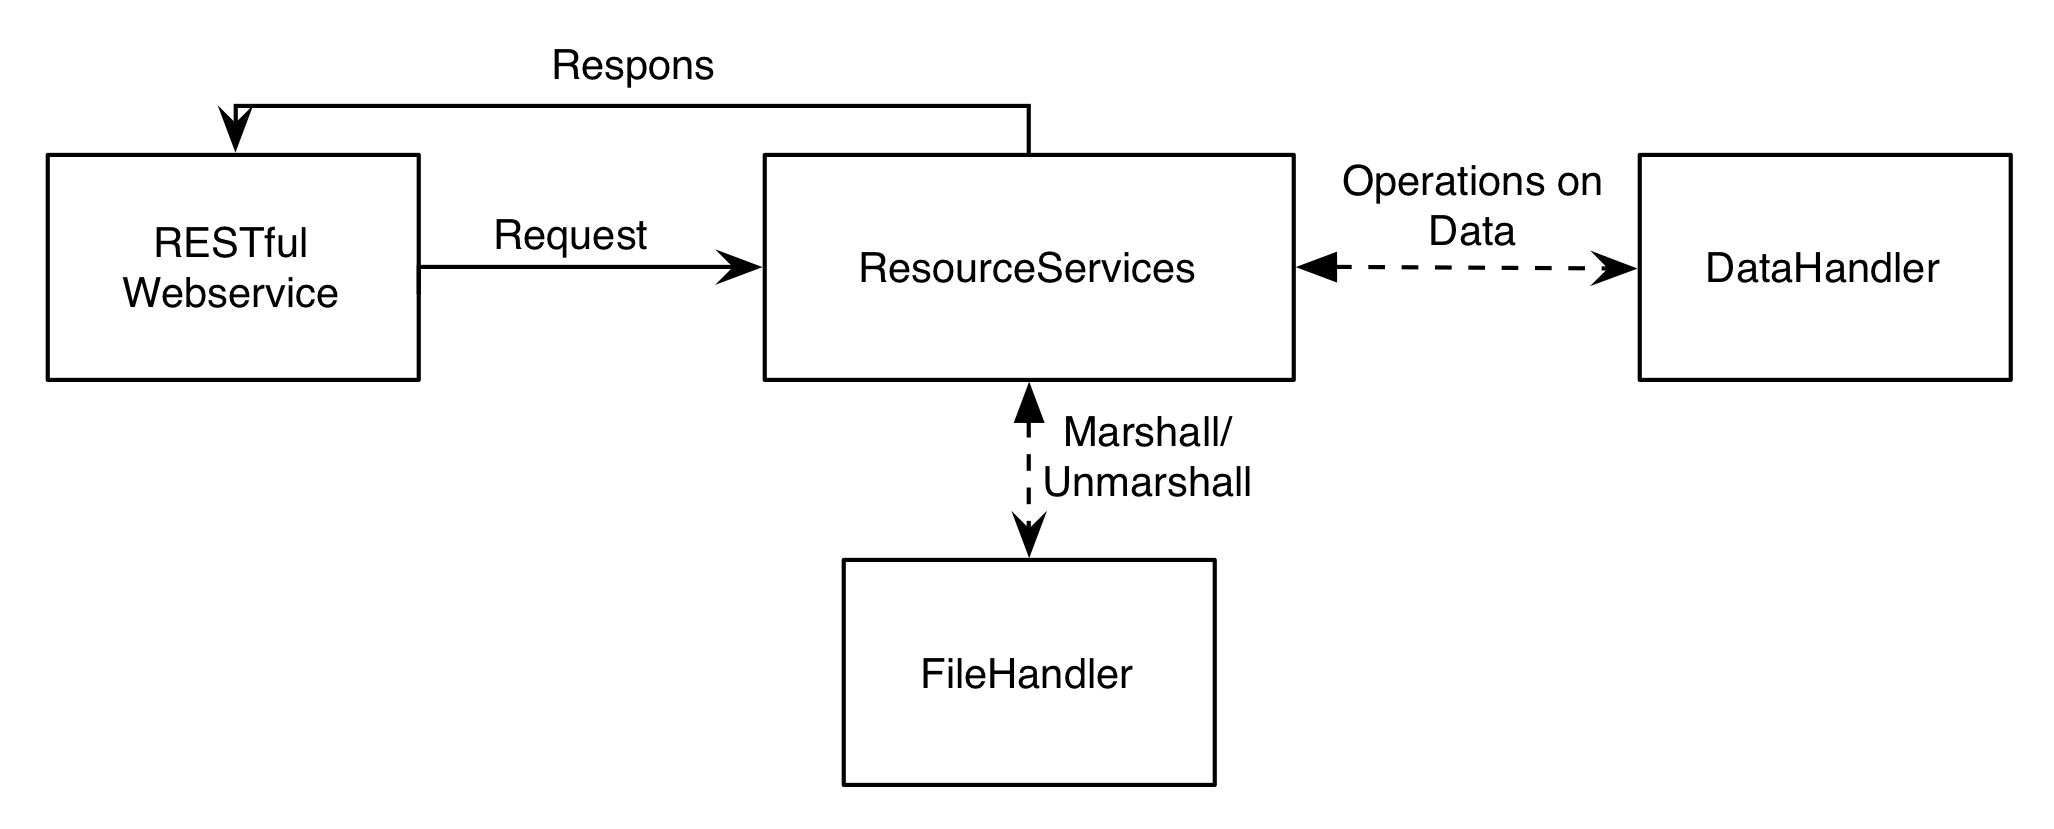
\includegraphics[width=1\textwidth]{images/aufbaurest.png}
\caption{Funktionaler Aufbau der Komponenten zur synchrone Kommunikation }
\label{RESTaufbau}
\end{figure}

TODO

\newpage

\subsection{Konzeption + XMPP Server einrichten}
Leafs (Topics) sollen für das Projekte definiert werden

Wer ist dabei Publisher und wer Subscriber?

Welche Daten sollen übetragen werden?

Entity
A JID-addressable Jabber entity (client, service, application, etc.).

Leaf Node
A type of node that contains published items only. It is NOT a container for other nodes.

Node
A virtual location to which information can be published and from which event notifications and/or payloads can be received (in other pubsub systems, this may be labelled a topic).

NodeID
The unique identifier for a node within the context of a pubsub service. The NodeID is either supplied by the node creator or generated by the pubsub service (if the node creator requests an Instant Node). The NodeID MAY have semantic meaning (e.g., in some systems or in pubsub profiles such as PEP the NodeID might be an XML namespace for the associated payload), but such meaning is OPTIONAL. If a document defines a given NodeID as unique within the realm of XMPP pubsub systems, it MUST specify the XML namespace of the associated payload.

Payload
The XML data that is contained within the <item/> element of a publication request or an event notification. A given payload is defined by an XML namespace and associated schema. A document that defines a payload format SHOULD specify whether the payload can be used only for a NodeID whose value is the same as the XML namespace, or whether the payload can be used for any NodeID. Such a document also SHOULD specify whether it is suggested that node at which such payloads are published are best configured as Singleton Nodes.

Publisher
Subscriber

Unterschiedliche Bedeutung von Node:
Service Discovery: Bereich der XMPP Entität, der den Umgang mit Anfragen und die Antwort bezüglich bestimmte Protokolle regelt.

<iq type='get'
    from='romeo@montague.nnet/orchard'
    to='mim.shakespeare.lit'
    id='info3'>
  <query xmlns='http://jabber.org/protocol/disco\#info' 
         node='http://jabber.org/protocol/commands'/>
</iq>
    


Publish Subscribe: Bestimmter Feed oder Channel, der in einem PubSub Service gehostet wird. Die Art des Channels wird durch den Payload charakterisiert.


<iq type='set'  
    from='hamlet@denmark.lit/blogbot'  
    to='pubsub.shakespeare.lit'  
    id='pub1'>  
  <pubsub xmlns='http://jabber.org/protocol/pubsub'>  
    <publish node='princely\_musings'>  
      <item>  
        <entry xmlns='http://www.w3.org/2005/Atom'>  
          <title>Soliloquy</title>  
          <summary>  
To be, or not to be: that is the question:  
Whether 'tis nobler in the mind to suffer  
The slings and arrows of outrageous fortune,  
Or to take arms against a sea of troubles,  
And by opposing end them?  
          </summary>  
          <link rel='alternate' type='text/html'  
                href='http://denmark.lit/2003/12/13/atom03'/>  
          <id>tag:denmark.lit,2003:entry-32397</id>  
          <published>2003-12-13T18:30:02Z</published>  
          <updated>2003-12-13T18:30:02Z</updated>  
        </entry>  
      </item>  
    </publish>  
  </pubsub>  
</iq>  




\newpage

\subsection{XMPP - Client}

Es soll ein XMPP Client entwickelt werden, dafür soll folgendes berücksichtigt werden:

Mittels der Anwendung soll es möglich sein Leafs zu abonnieren, Nachrichten zu empfangen und zu veröffentlichen.
Ermöglichen Sie die Übertragung von Nutzdaten (Beispielsweise Simplepayload)
Leafs und ggf. mögliche Eigenschaften der Leafs sollen angezeigt werden können (Service Discovery)
Service Discovery, disco: definiert in XEP-0030, 
2 wesentliche Methoden: disco\#items -> discover entities; disco\#info -> welche features werden von einer Entität unterstüzt

disco\#items: IQ-get an server gesendet, Replie liste der verbundenen EntitiesSimplepayload




\newpage

\subsection{Client - Entwicklung}
\subsubsection{Vorbereitung und Layoutentwicklung}
Im finalen Meilenstein des Projektes, steht die Entwicklung eines grafischen Userinterface im Mittelpunkt, der die Funktionalität des Systems repräsentiert. Die Applikation soll die entsprechende Verbindung zum Server aufbauen und den Datenaustausch ermöglichen. \\

Vor der praktischen Umsetzung mit Java Swing, wurde ein mögliches Konzeptlayout erstellt und entsprechende Alternativen ausprobiert.Hierbei handelt es sich um erste Ideen wie die Anwendung aufgebaut sein kann und welche Elemente benötigt werden.
Da in der letztendlichen Umsetzung aber hauptsächlich die Funktionalität im Mittelpunkt steht, wurde speziell darauf geachtet, dass alle Funktionalitäten in einem logischen Kontext eingebunden werden und anwendbar sind. Auf genaue Designkonzepte zum optimalen Aufbau wurde hierbei verzichtet, da sie im entsprechenden Projektkontext nicht an erster Stelle stehen sollten. In einem größer angelegten Projekt sollte hierbei eine intensivere Auseinandersetzung folgen mit entsprechender Validierung und Testdurchläufe. \\

Die Applikation soll mit einer Startseite (Abb. 4a) beginnen, von der aus der Anwender die Möglichkeit hat sich zu identifizieren. Entweder er meldet sich mit bereits vorhandenen Daten an oder er registriert sich als neuer Benutzer.
Sind bereits Accountdaten vorhanden, so folgt eine Eingabe des Usernamen und des Passworts (Abb. 4b). Sollte der User eine der beiden Informationen vergessen haben, so besteht die Option \textit{Passwort/Username vergessen?}, wobei die funktionale Implementierung nicht stattfinden wird und dies eher als Platzhalter dient. Nach Eingabe der Daten und Prüfung auf Korrektheit, wird zur \textit{Homeseite} weitergeleitet, die als Hauptseite dient und von der aus die verschiedenen Funktionen angesteuert werden.

\begin{figure}[h!]
\centering
\hfill %
\subfloat[Startseite \label{pic:Anmelden}]{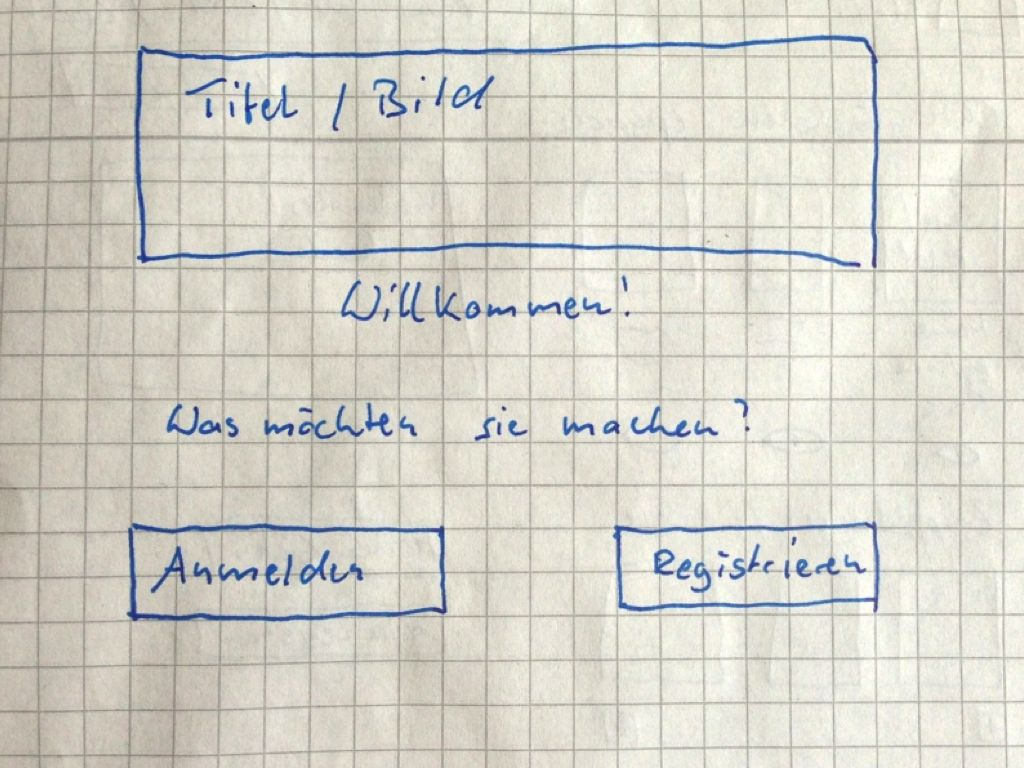
\includegraphics[width=.5\textwidth]{images/dokulayout/startseite.jpg}}
\hfill % alternativ auch \hspace{1cm} für genaue Angaben
\subfloat[Einloggen \label{pic:Registrieren}]{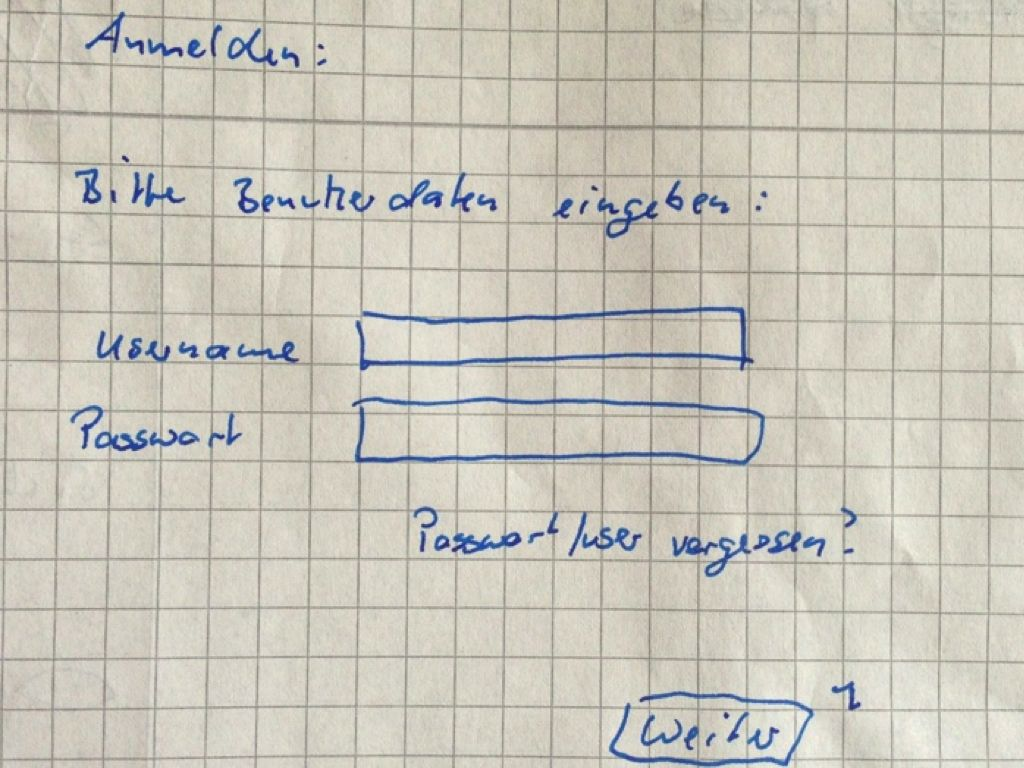
\includegraphics[width=.5\textwidth]{images/dokulayout/anmelden.jpg}}
\hfill %
\caption{Gui Layout Skizzen: Startauswahl und Einloggen }
\label{Gui}
\end{figure}




\newpage

Entscheidet man sich für die Auswahl \textit{Registrieren} wird ein neuer Account angelegt. Auf der ersten Seite (Abb. 5a) werden die Grundinformationen eingegeben, wobei hier nur Username und Passwort und Name notwendig sind und die zusätzlichen Informationen jederzeit ergänzt werden können. Nach Eingabe und Kontrolle folgt der zweite Teil der Registrierung, die Auswahl der Genreprioritäten (Abb. 5b). Da der Serientracker die Option anbietet, Informationen zu Serien eines bestimtmen Genres zu erhalten, dient dieser Schritt dazu bestimmte Genres zu abonnieren. Auch hier soll die Auswahl später geändert werden können.\\

\begin{figure}[h!]
\centering
\hfill 
\subfloat[Registrieren \label{pic:Registrieren}]{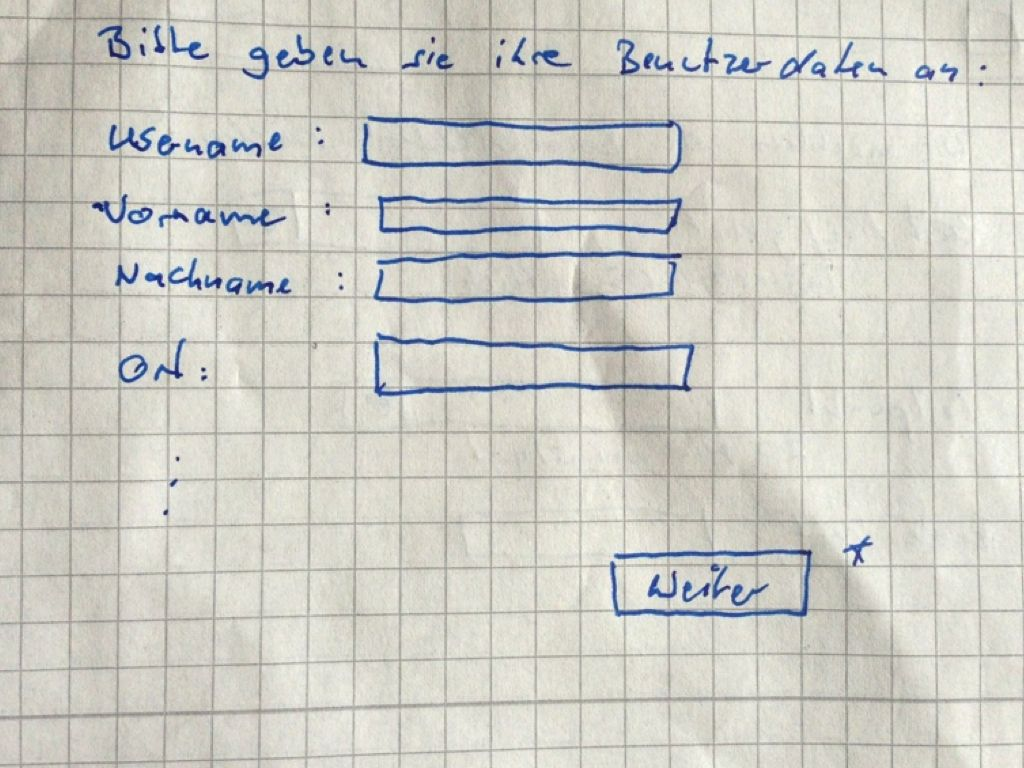
\includegraphics[width=.5\textwidth]{images/dokulayout/registrieren.jpg}}
\hfill % alternativ auch \hspace{1cm} für genaue Angaben
\subfloat[Prioritäten \label{pic:Prioritaeten}]{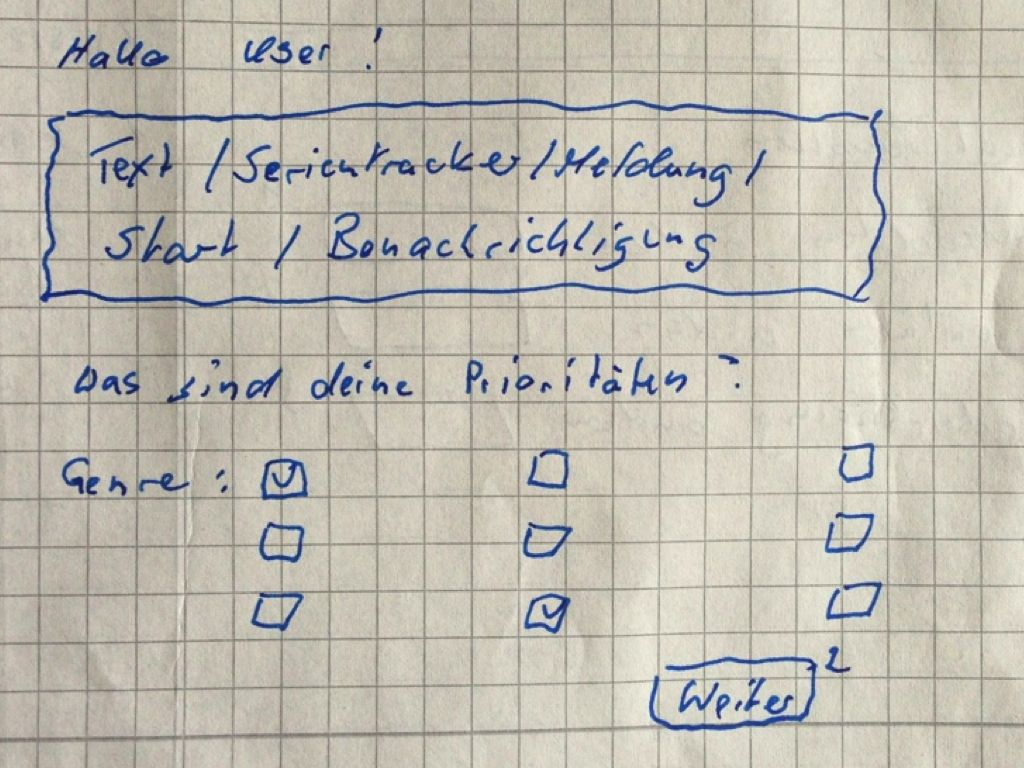
\includegraphics[width=.5\textwidth]{images/dokulayout/prioritaeten.jpg}}
\hfill %
\caption{Gui Layout Skizzen: Registrierung }
\label{Gui}
\end{figure}

\parskip 12pt
\parindent 0pt


\begin{wrapfigure}{r}{0cm}
\centering
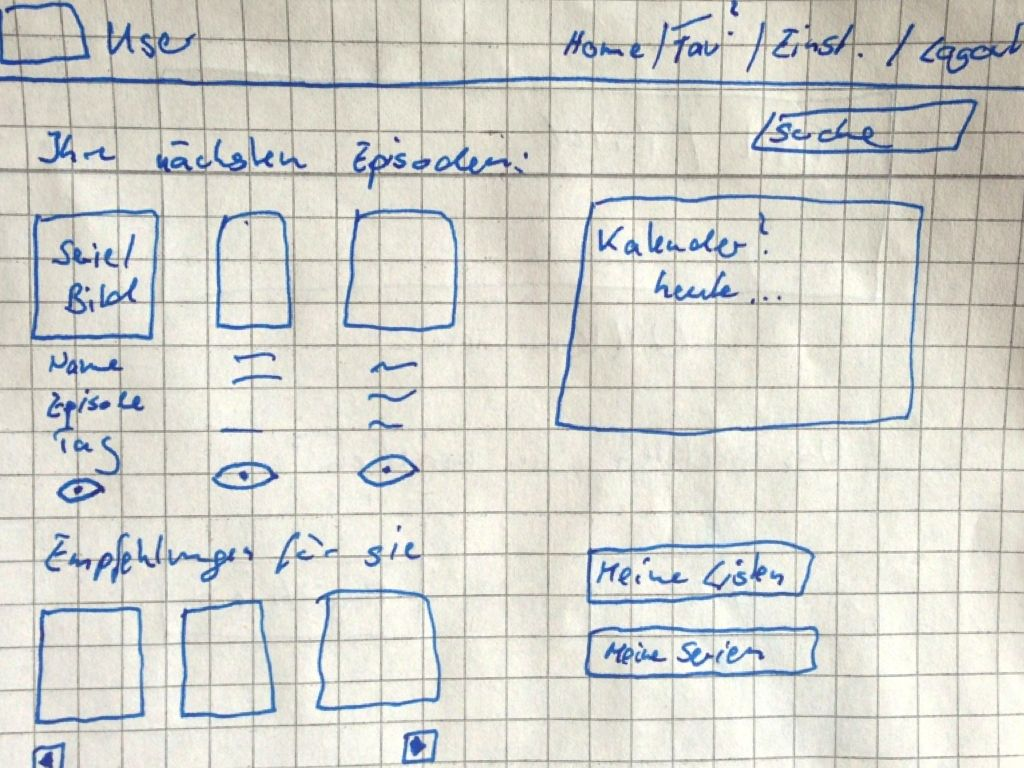
\includegraphics[width=.5\textwidth]{images/dokulayout/home.jpg}
\caption{Gui Skizzen: Homeansicht}
\end{wrapfigure}

Nach erfolgreicher Identifizierung des Users folgt der Homebereich (Abb. 6). Dies ist der eigentliche Ausgangspunkt für alle Aktivitäten und dient als Benutzerzentrale. Am oberen Bereich findet sich eine statische Menüleiste, die sich in diesem Aufbau durch alle weiteren Bereiche zieht und jederzeit zugänglich ist. Information zum angemeldeten User und die Optionen \textit{Home}, \textit{Favoriten}, \textit{Einstellung}und\textit {Logout}. Home führt jederzeite zur Hauptübersicht, Einstellung ermöglicht entsprechende Möglichkeiten zur Accountverwaltung und Logout meldet den aktuellen Benutzer ab und führt wieder zur Anmeldung. Die Option Favoriten war als Verwaltung zu den angelegten Lieblingsgenre geplant, wurde aber in weiteren Entwürfen in die Einstellungen mit eingebunden, da bis auf eine einfache Auswahl kein größerer Nutzen für den User angeboten wird. Für den Fall das Adminrechte vorhanden sind, wurde in einem späteren Entwurf der zusätzliche Menüpunkt \textit{Hinzufügen} eingebunden. Dort lassen sich neue Serien, Staffeln, Episoden und Genrelisten anlegen. \\


\newpage 

Da im Mittelpunkt des Konzeptes die Benachrichtigung über neue Episoden steht, werden dem User bereits nach einloggen die wichtigsten Informationen präsentiert. Neben einer Suche, werden die Ausstrahlungszeitpunkte der nächsten Episoden angezeigt. Neben dieser Übersicht sollten zudem direkte Benachrichtigungen in Form von Pop-Ups stattfinden, weshalb diese Ansicht vorallem der Erinnerung und Verwaltung dient. Inwiefern eine Darstellung der heutigen Serien in Form eines Kalender realisierbar wäre ist zur Zeit der Konzipierung noch unklar, sollte aber eher als \textit{nice-to-have Feature} betrachtet werden.\\
Dazu gab es die Überlegung Serienempfehlung zu geben, basiernd auf abonnierten Genres. Buttons zu \textit{Meine Serien} und \textit{Meine Listen} führen zu entsprechenden Unterkategoerien.
Meine Serien zeigt einer Auflistung der Serien über die man Benachrichtigungen erhalten möchte und die derzeit angeschaut werden. Meine Listen gibt einen Überblick über angelegte Listen zur Ordnung von Serien nach bestimmten Themen und bietet zudem die Möglichkeit eine neue Liste anzulegen. \\

\parskip 12pt
\parindent 0pt

Nach Auswahl einer bestimmten Serie werden vorhandene Information präsentiert. Allgemeine Informationen, eine Übersicht zu vorhandenen Staffeln und eine Darstellung der nächsten Episode die Ausgestrahlt wird und gegebenfalls die Episode die der Benuter zuletzt gesehen hat. Hierbei würde die Verwaltung mit Hilfe der Seen List stattfinden, wobei auch hier die letztendliche Umsetzung eher unwahrscheinlich ist.
Auf dieser Seite (Abb. 7a) kann die Serie einer bestimmten Liste hinzugefügt werden und wird damit abonniert. In einer weiteren Variante der Serienseite (Abb. 7b) handelt es sich um die Darstellung unter Adminrechte, wobei die \textit{Add to List} Option nun zum Editieren dieser Seite führt und auch neben den Serien eine entsprechende Editierfunktion eingeführt wird. 

\begin{figure} [h!]
\centering
\hfill %
\subfloat[Serienseite User \label{pic:Serienseite}]{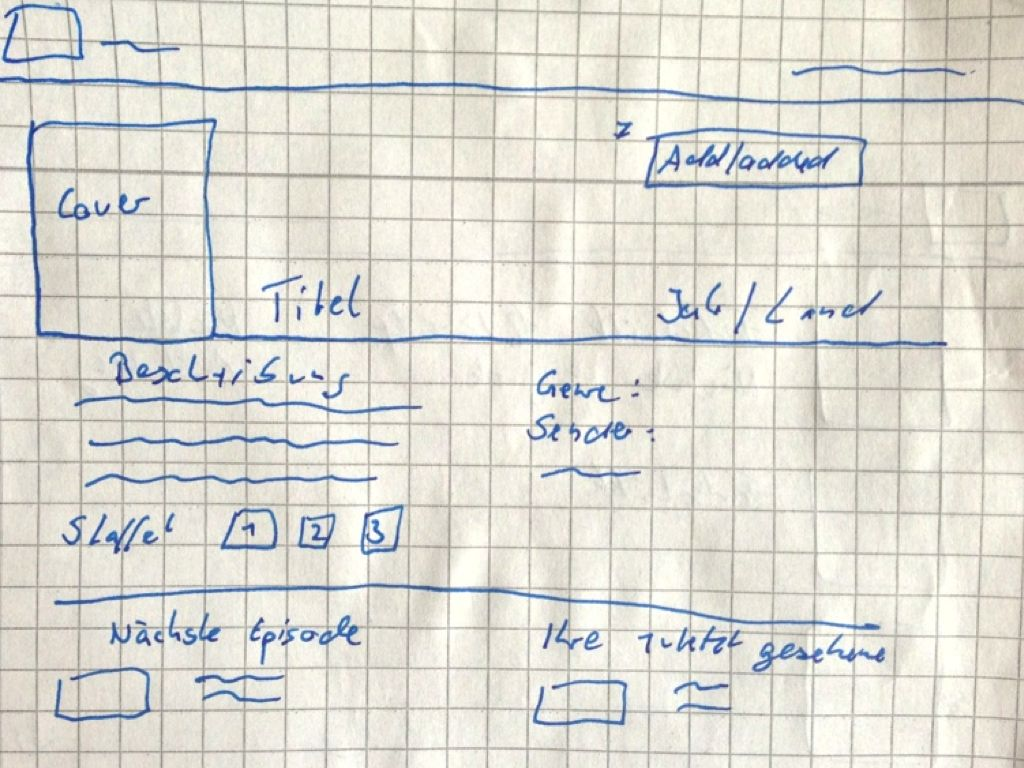
\includegraphics[width=.5\textwidth]{images/dokulayout/serie.jpg}}
\hfill % alternativ auch \hspace{1cm} für genaue Angaben
\subfloat[Serienseite Admin \label{pic:Serienseite}]{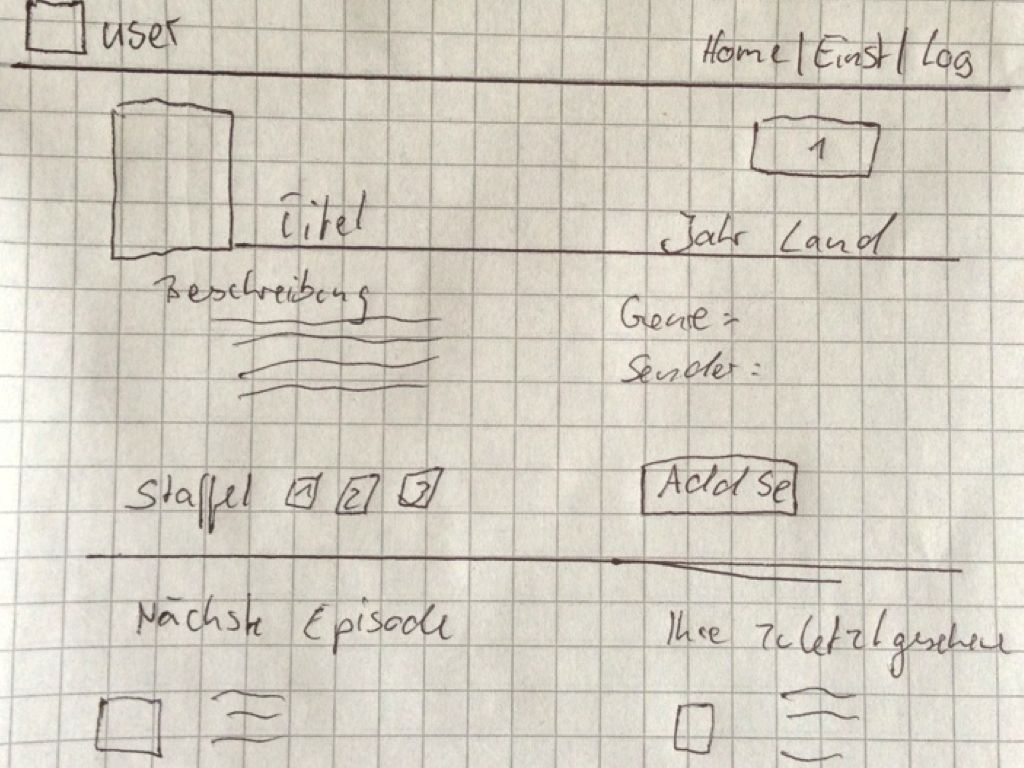
\includegraphics[width=.5\textwidth]{images/dokulayout/serie2.jpg}}
\hfill %
\caption{Gui Layout Skizzen: Serienübersicht }
\label{Gui}
\end{figure}





\newpage 

Die jeweilige Seasonseite (Abb. 8a) zeigt eine Vorschau zu vorhandenen Episoden und bietet dem Admin erneut die \textit{Add Episode} Funktion (Abb. 8b). In welcher Form die Episoden aufgeführt werden ist zu diesem Zeitpunkt noch nicht festgelegt und wird bei entsprechender Umsetzung entschieden. Wird eine neue Episode angelegt (Abb. 8b) wird entsprechende Serie und Staffel referenziert und die einzelnrn Informationen eingegeben.\\
\begin{figure} [h!]
\centering
\hfill %
\subfloat[Seasonseite \label{pic:Seasonseite}]{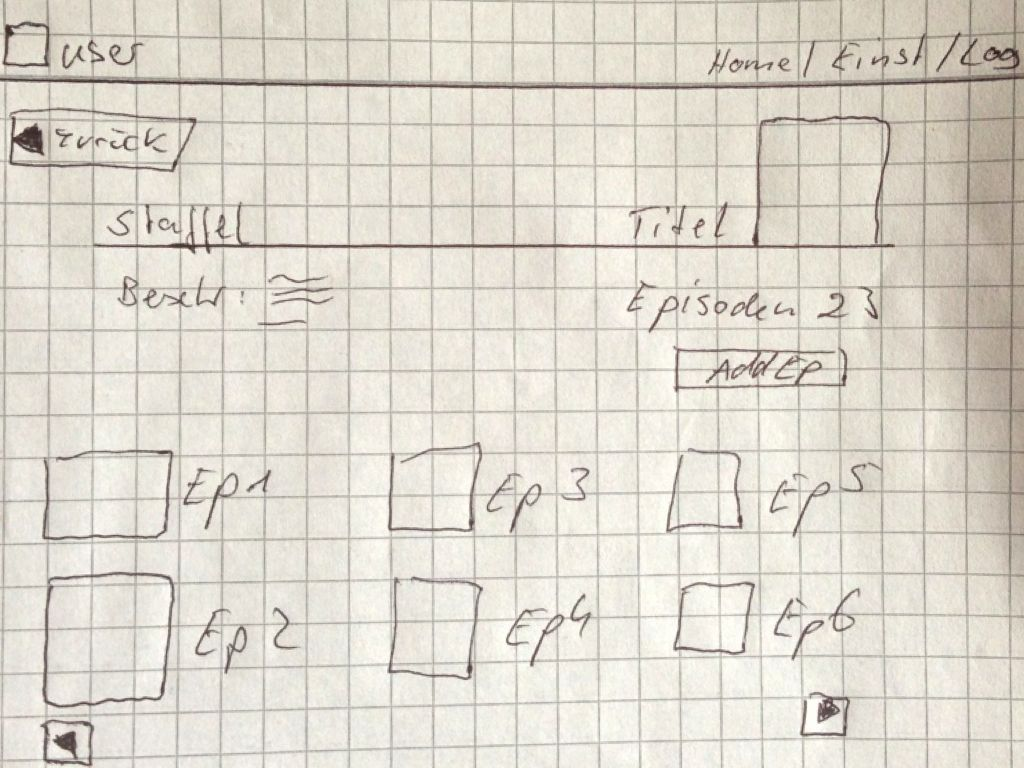
\includegraphics[width=.5\textwidth]{images/dokulayout/staffel.jpg}}
\hfill % alternativ auch \hspace{1cm} für genaue Angaben
\subfloat[Episode anlegen \label{pic:Episodenverwaltung}]{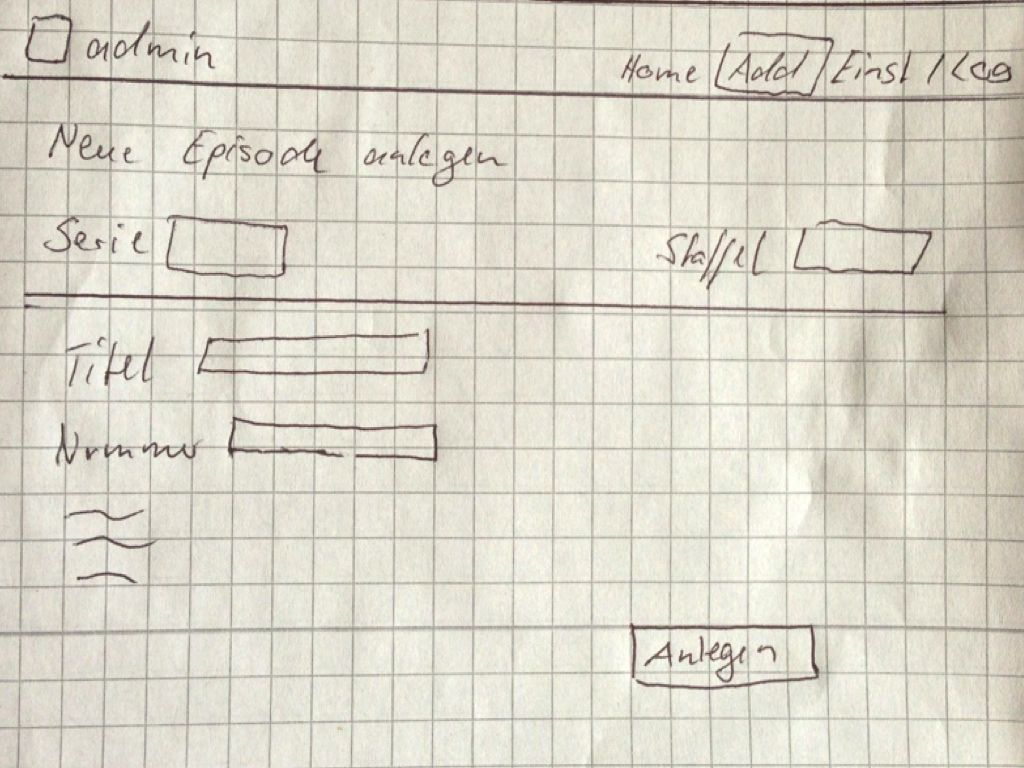
\includegraphics[width=.5\textwidth]{images/dokulayout/anlegen.jpg}}
\hfill %
\caption{Gui Layout Skizzen: Seasonübersicht und Verwaltung }
\label{Gui}
\end{figure}

Bei der Planung der GUI, wurden die einzelnen Seiten nach entsprechenden Ideen konzipiert und weiterentwickelt. Die vorgestellten Entwürfe sollten einen kurzen Einblick in die Planungsphase geben und dienten in dieser Form keiner finalen Vorlage, nach der die Entwicklung stattfindet. Aus diesem Grund wird hier im weiteren nicht auf jede einzelne Unterseite eingegangen.\\ Während bei den ersten Varianten vorallem der mögliche Aufbau und die Darstellung der einzelnen Elemente im Vordergrund stand, wurden in späteren Versionen speziell auf entsprechende Funktionalität und Verweisen geachtet. Dabei entstand unter anderem die Adminansicht, welche die Kategorien um verwaltende Optionen erweitert. Ob jede Vorstellung realisierbar bzw. im Projektkontext notwendig ist und wie sich entsprechendes Layout letztendlich entwickelt hat, wird in der Umsetzung dargestellt. (Diesen Absatz eventuell überarbeiten, noch nicht ganz passend) \\



\newpage
\subsubsection{Umsetzung}



\newpage

\section{Projektreflektion}

\newpage

\listoffigures

\newpage 

\listoftables


\end{document}
